\documentclass[10pt,a4paper]{beamer}
\usepackage[latin1]{inputenc}
\usepackage[spanish]{babel}
\usepackage[T1]{fontenc}
\usepackage{amsmath}
\usepackage{amsfonts}
\usepackage{amssymb}
\usepackage{graphicx}
\usepackage{beamerthemesplit}
\usepackage{float}
\usepackage{multirow}
\usepackage{multicol}
\usepackage{url}
\usepackage{ragged2e}
\usepackage{array}
\usepackage{latexsym}
\usepackage{subfigure}
\usepackage{timing}
\usepackage{url}

\setbeamertemplate{footline}[frame number]
\setbeamertemplate{bibliography item}[text]
%\setbeamertemplate{subsubsection in sidebar shaded}
%{\tableofcontents[subsubsectionstyle=hide]}

%\usetheme{Montpellier}
\usetheme{Warsaw}
\decimalpoint
\renewcommand{\contentsname}{Contenido}

\begin{document}

\title{Integraci�n sem�ntica de \\ los recursos de informaci�n en \\ una memoria corporativa}
\author{Erik Alarc�n Zamora}
\date{Enero 2014. M�xico, D.F.}

\begin{frame}
\titlepage
\centering
Asesores:\\ Dra. Reyna Carolina Medina Ram�rez \\Dr. H�ctor P�rez Urbina
\\
\end{frame}
\begin{frame}
\frametitle{Contenido}
\setcounter{tocdepth}{1}  
\begin{scriptsize}\tableofcontents[]\end{scriptsize}
\end{frame}
\section{Marco Introductorio}

\subsection{Contexto y Motivaci�n}

\subsubsection{Memoria Corporativa}
\begin{frame}[allowframebreaks]
	\frametitle{Memoria Corporativa}
	%%%%%%%%%%%%%%%%%%%%%%%
	\begin{block}{Definici�n}
	\justifying 
	La representaci�n expl�cita, t�cita, consistente y persistente del conocimiento de una organizaci�n. \cite{Ontoinra2002}
	\end{block}
	
	\begin{block}{Finalidad}
	\justifying 
	Una memoria corporativa conserva y mantiene el conocimiento de una organizaci�n \cite{Corpmem98}, para \textit{facilitar el acceso, intercambio y difusi�n de �ste}.
	\end{block}
	
	\begin{exampleblock}{Caso de Estudio}
	\justifying 
	El grupo de investigaci�n del �rea de Redes y Telecomunicaciones (RyT) de la Universidad Aut�noma Metropolitana Unidad Iztapalapa (UAM-I).
	\end{exampleblock}
	%%%%%%%%%%%%%%%%%%%%%%%
	
	\begin{block}{Recurso de Informaci�n}
	\justifying 
	Un elemento que representa y encapsula una parte del conocimiento de una organizaci�n (investigaciones, colaboraciones, proyectos, cursos, temas de inter�s, objetos e ideas).
	\end{block}
	
	\begin{figure}[htbp]
	\centering
	\subfigure[Conocimiento del �rea de RyT]{
	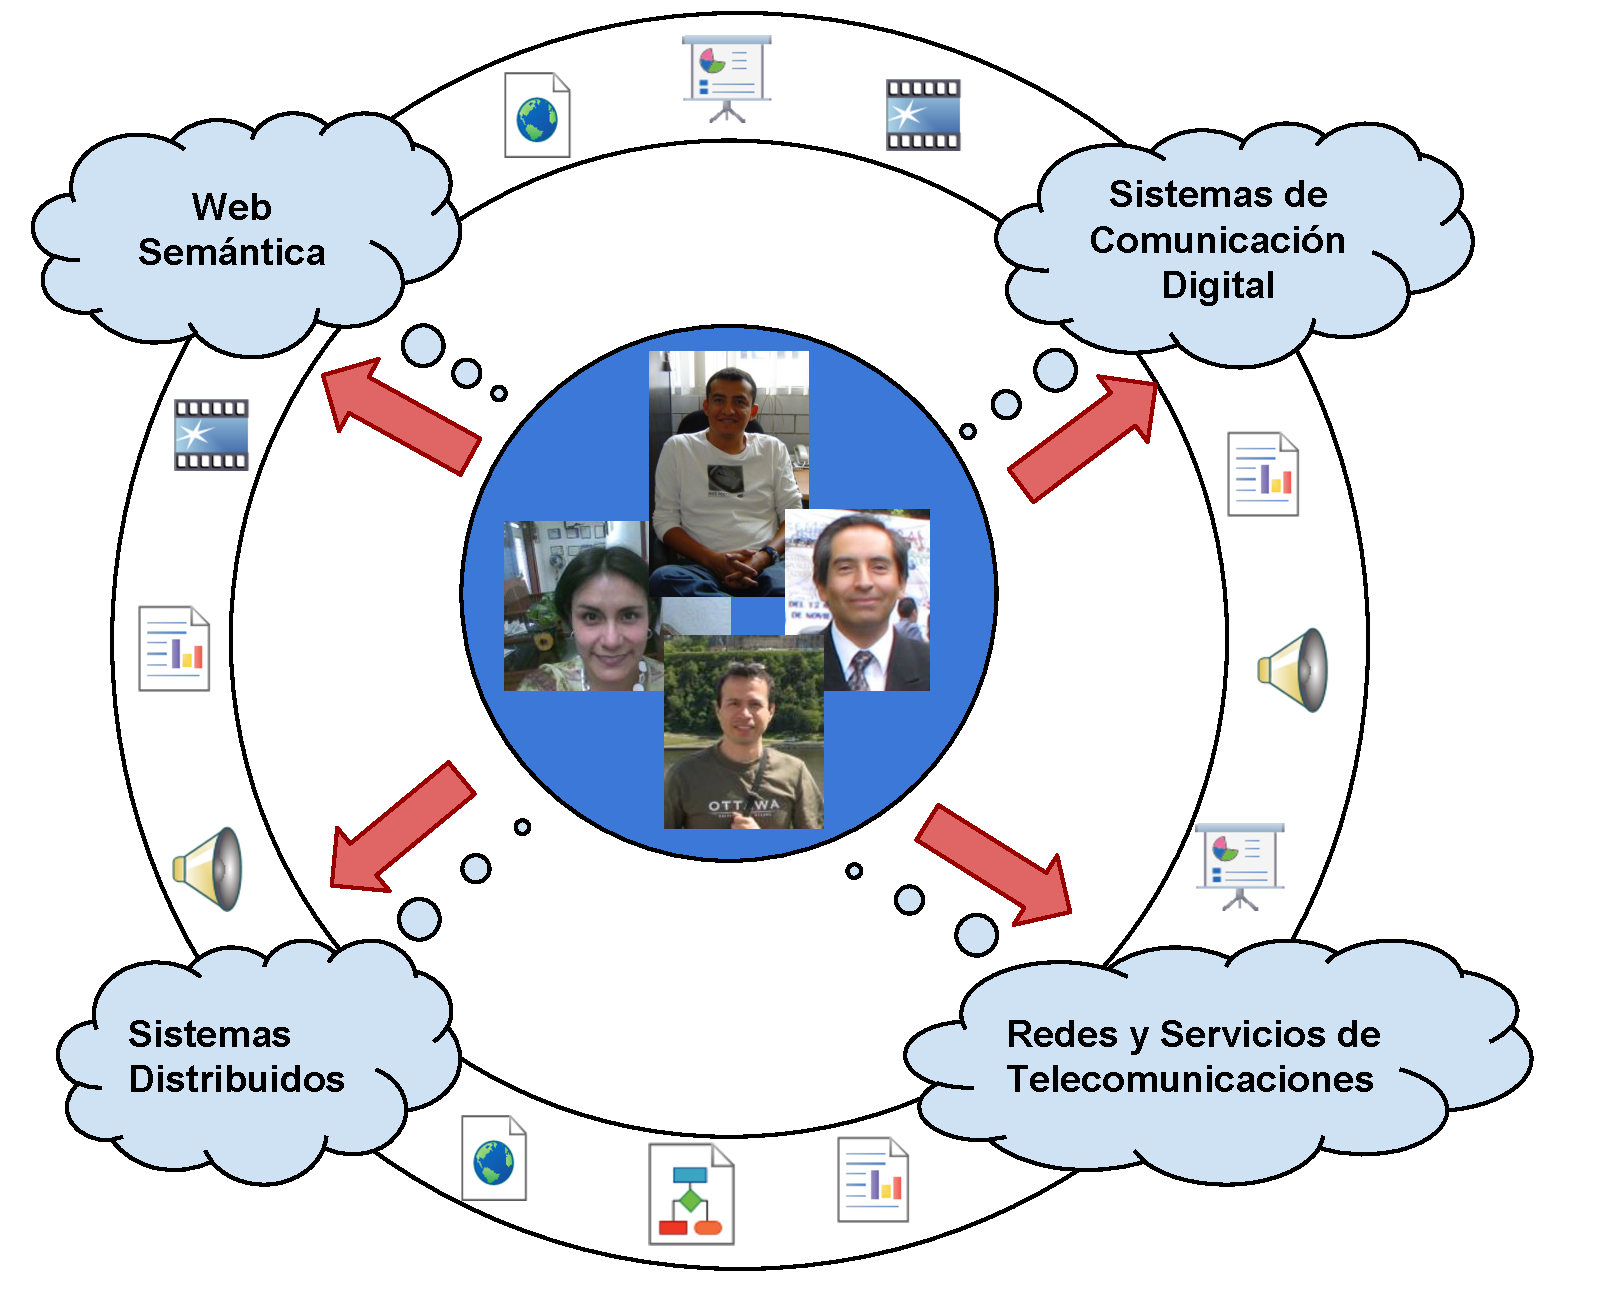
\includegraphics[scale=0.17]{ConocimientoRyT} 
	}
	\subfigure[Memoria Corporativa del �rea de RyT]{
	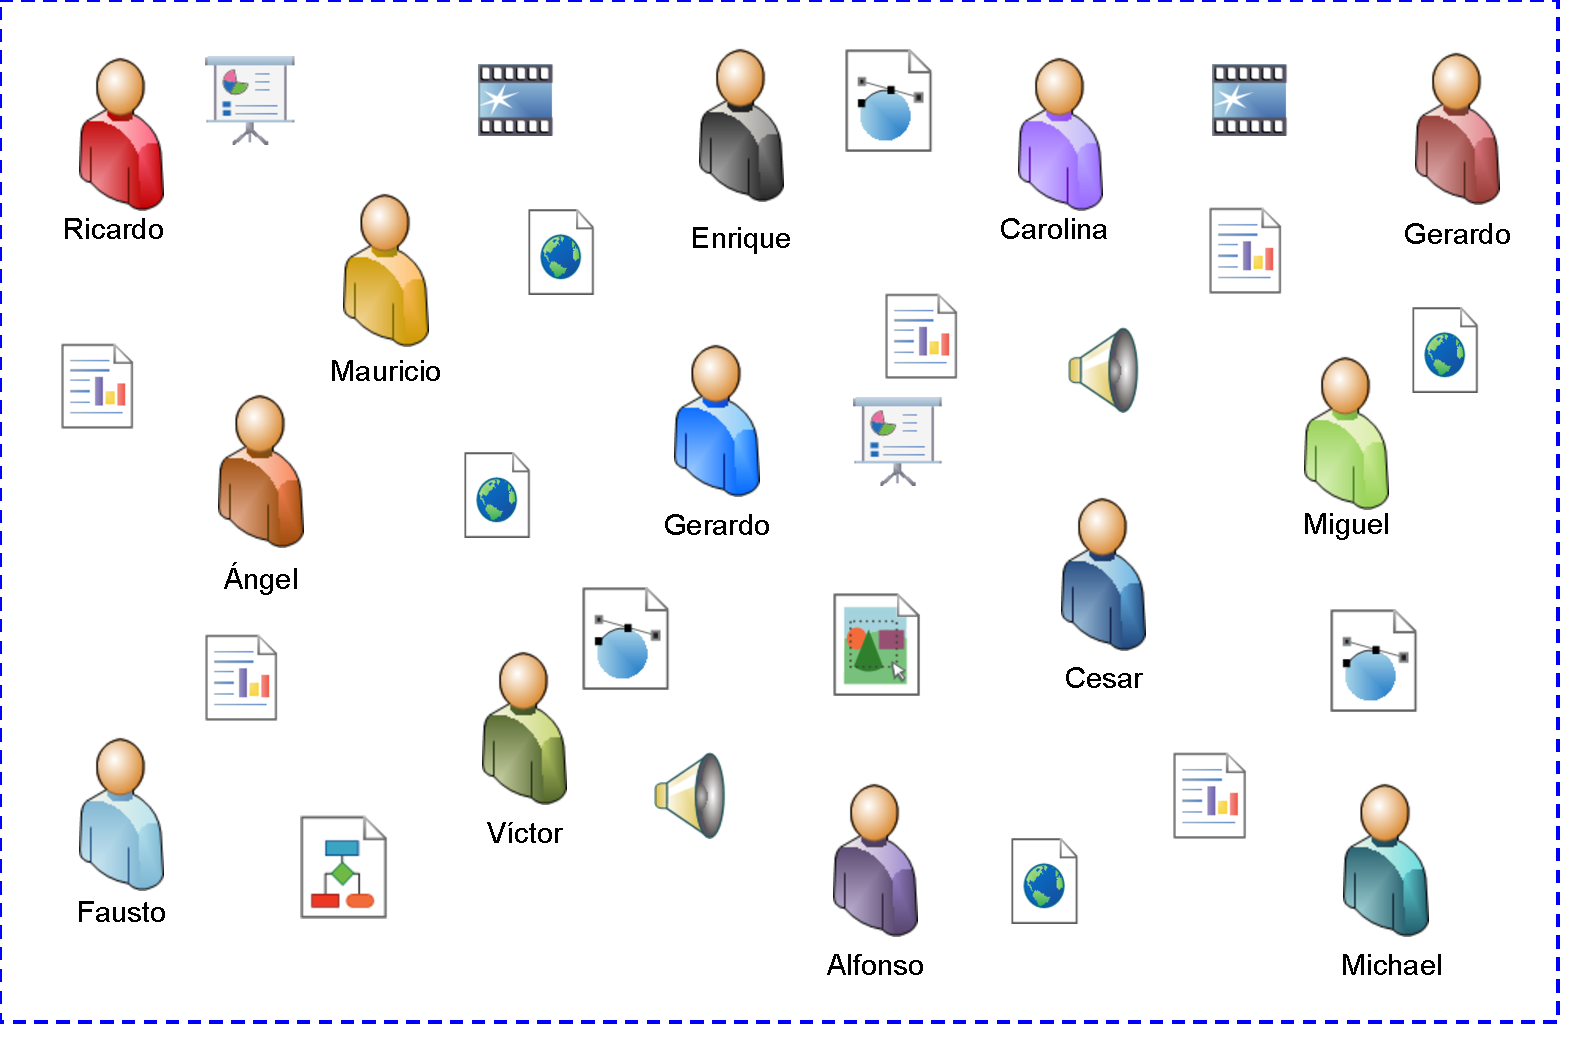
\includegraphics[scale=0.18]{EjemploMC} 
	}
	\end{figure}
	%%%%%%%%%%%%%%%%%%%%%%%
	
	\begin{figure}
	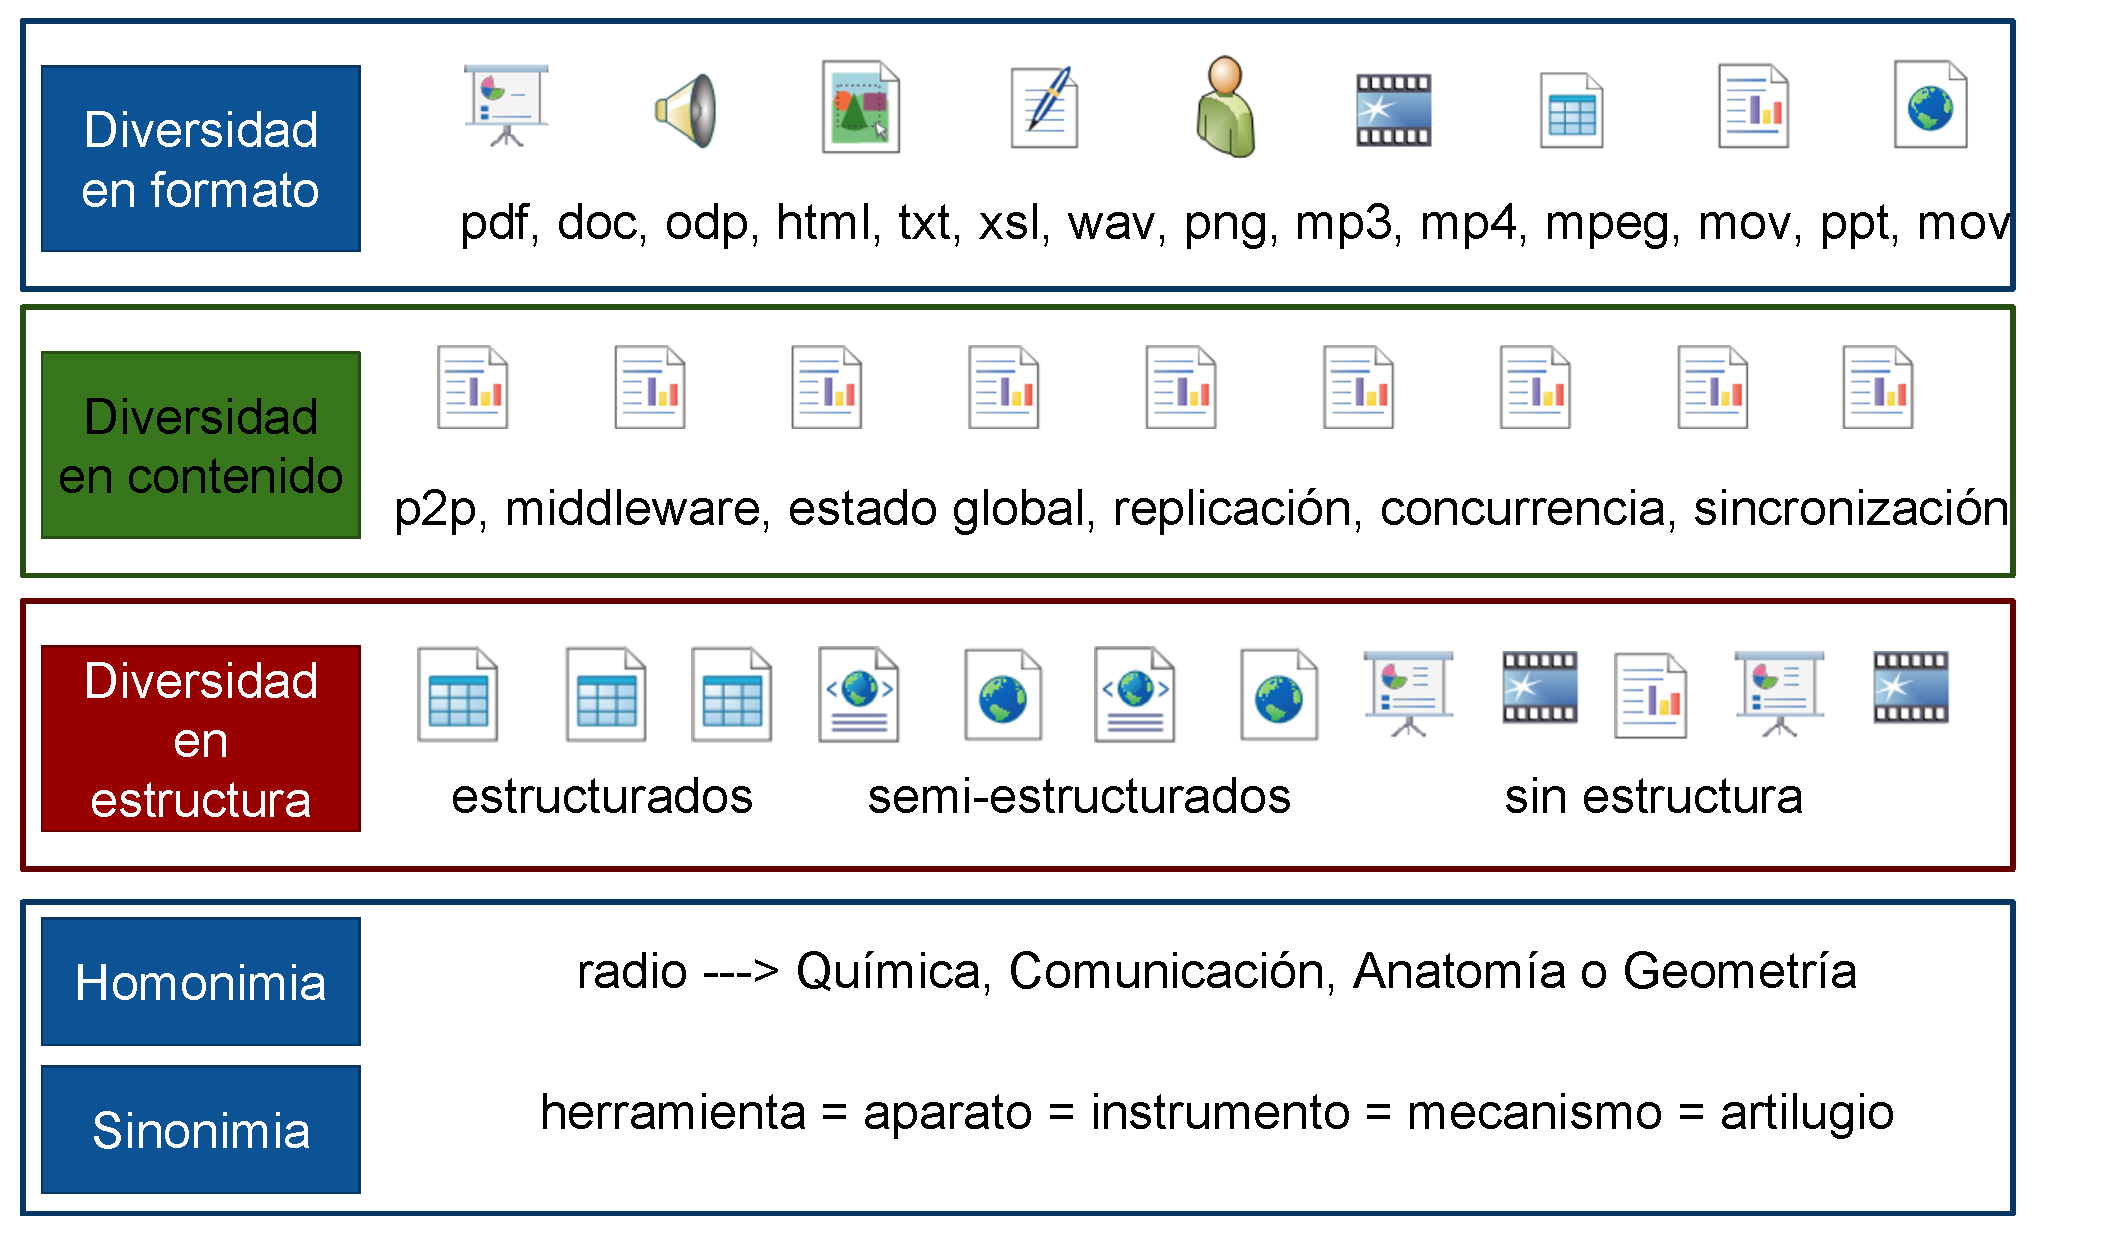
\includegraphics[scale=0.33]{NatMC} 
	\end{figure}
	%%%%%%%%%%%%%%%%%%%%%%%
\end{frame}

\subsubsection{Tecnolog�as Sem�nticas}
\begin{frame}[allowframebreaks]
	\frametitle{Tecnolog�as Sem�nticas}
	%%%%%%%%%%%%%%%%%%%%%%%
	\begin{block}{Definici�n}
	\justifying 
	\textit{Un conjunto de metodolog�as, lenguajes, aplicaciones, herramientas y est�ndares para suministrar u obtener el significado de las palabras, informaci�n y las relaciones entre �stos}. \begin{scriptsize}\cite{SemTecRetr}\end{scriptsize}
	\end{block}
	
	\begin{figure}
	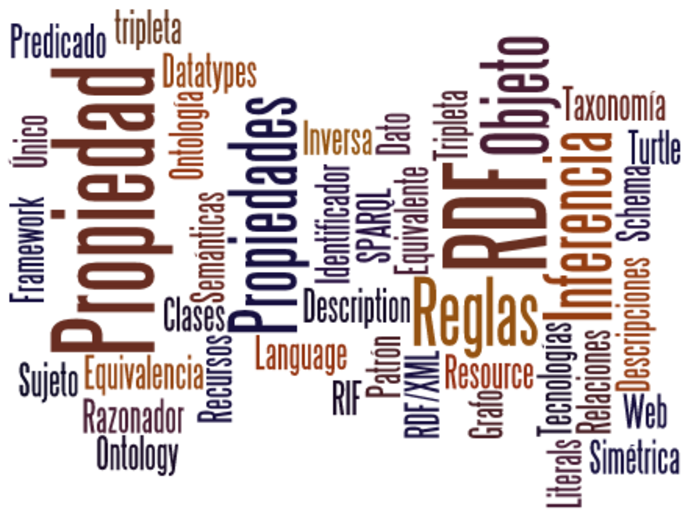
\includegraphics[scale=0.42]{TSWords} 
	\end{figure}
	%%%%%%%%%%%%%%%%%%%%%%%
	
	\begin{block}{Resource Description Framework (RDF)}
	\justifying 
	Marco gen�rico para describir el conocimiento e informaci�n expl�cita de los recursos mediante sus caracter�sticas y relaciones. \begin{scriptsize}\cite{SurvSemWeb2012}\end{scriptsize}
	\end{block}
	
	\begin{block}{Recurso}
	\justifying 
	Puede ser cualquier cosa (persona, lugar, documento, entidades del mundo real o conceptos abstractos) que tiene un identificador �nico de recursos (URI).
	\end{block}
	
	\begin{block}{Propiedad}
	\justifying 
	Un aspecto significativo, caracter�stica, o relaci�n que se describe de un recurso (relaci�n binarias).
	\end{block}
	%%%%%%%%%%%%%%%%%%%%%%%
	
	\begin{block}{Clase}
	\justifying 
	Una colecci�n de objetos que comparten caracter�sticas comunes.
	\end{block}
	
	\begin{block}{Literal}
	\justifying 
	Un valor de datos como cadenas o enteros particulares.
	\end{block}
	
	\begin{block}{Declaraci�n}
	\justifying 
	Una afirmaci�n de un hecho expl�cito sobre un recurso, en t�rminos de una propiedad y el valor asignado a �sta.
	\begin{itemize}
	\item \justifying Juan se llama ``Juan L�pez Mart�ez''.
	\item \justifying Juan estudia en la UAM.
	\item \justifying Juan es un estudiante.
	\end{itemize}
	\end{block}
	%%%%%%%%%%%%%%%%%%%%%%%
	
	\begin{block}{Tripleta RDF}
	\justifying 
	La forma b�sica para representa una declaraci�n en un modelo sem�ntico.
	\end{block}
	
	\begin{figure}
	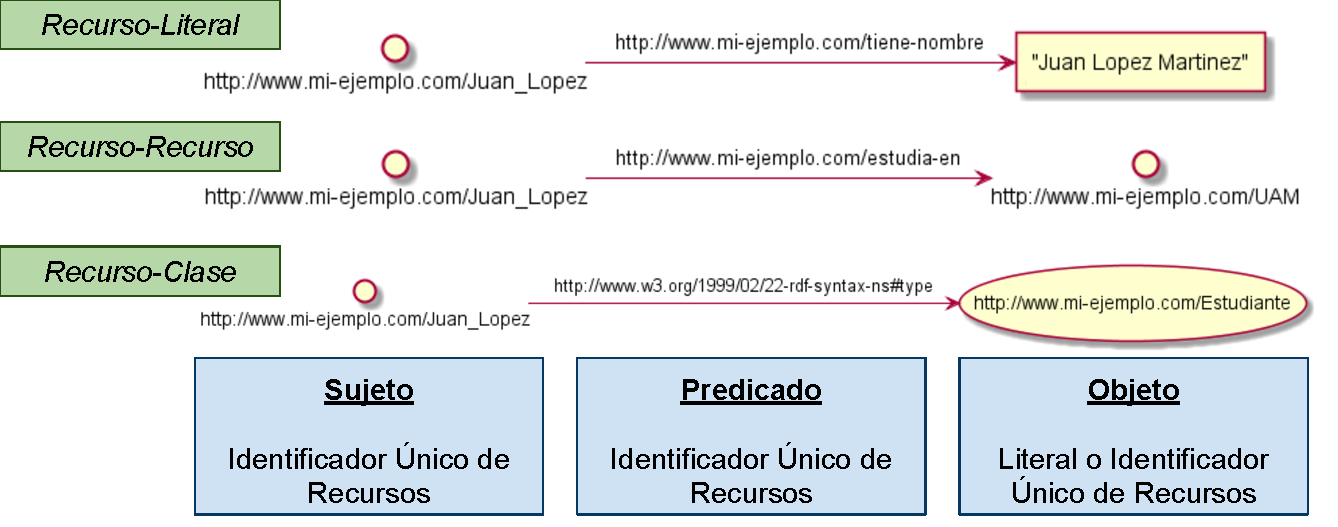
\includegraphics[scale=0.5]{Tripletas} 
	\end{figure}
	%%%%%%%%%%%%%%%%%%%%%%%
	
	\begin{block}{Grafo RDF}
	\justifying 
	Un grafo estructurado y dirigido compuesto por nodos, aristas y etiquetas para representar las tripletas.
	\end{block}
	
	\begin{figure}
	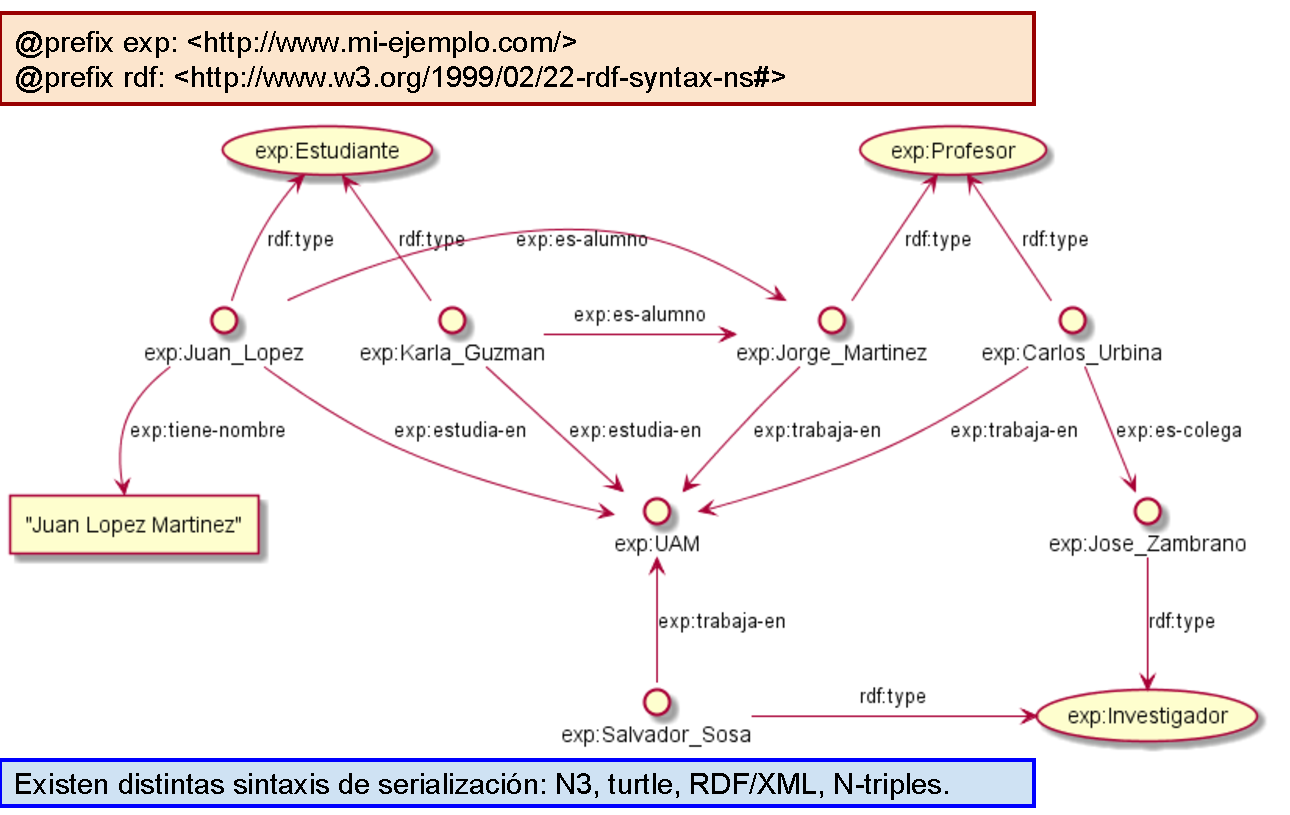
\includegraphics[scale=0.38]{GrafoRDF} 
	\end{figure}
	%%%%%%%%%%%%%%%%%%%%%%%
	
	\begin{block}{SPARQL}
	\justifying 
	Lenguaje de consulta y protocolo de acceso a RDF, para la b�squeda y recuperaci�n de la informaci�n en un grafo RDF.
	\end{block}
	
	\begin{block}{Motor de B�squeda SPARQL}
	\justifying 
	Programa que interpreta una consulta SPARQL, la compara con el grafo RDF y recupera los valores de la misma.
	\end{block}
	
	\begin{figure}
	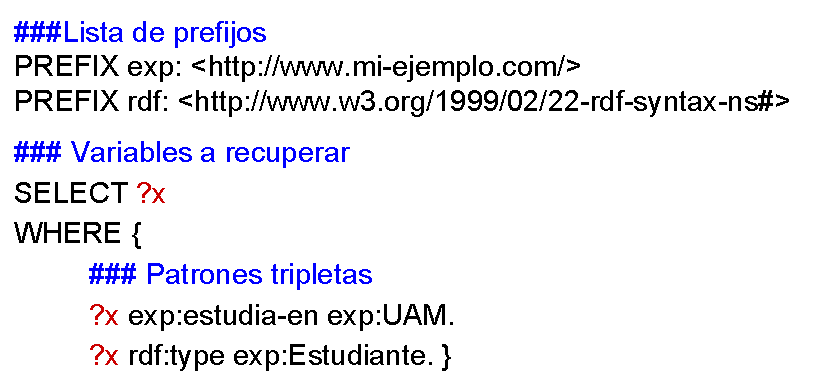
\includegraphics[scale=0.4]{FormaSPARQL} 
	\end{figure}
	%%%%%%%%%%%%%%%%%%%%%%%
	
	\begin{alertblock}{Ontolog�a}
	\justifying 
	Una definici�n formal, expl�cita y compartida de los conceptos, as� como las relaciones de un determinado dominio. \begin{scriptsize}\cite{Gruber}\end{scriptsize}
	\end{alertblock}
	
	\begin{block}{Componente Asertivo (ABox)}
	\justifying 
	Este componente est� constituido por las declaraciones (descripciones o hechos verdaderos) que afirman que los individuos son instancias de una clase o propiedad.
	\end{block}
	
	\begin{block}{Componente Terminol�gico (TBox)}
	\justifying 
	Este componente describe las clases y propiedades relevantes, as� como las reglas de inferencia que permiten aprovechar la manera en que las instancias se relacionan entre s�.
	\end{block}
	%%%%%%%%%%%%%%%%%%%%%%%
	
	\begin{block}{Reglas de inferencia o Axiomas}
	\justifying 
	 Los \textit{axiomas} o \textit{reglas de inferencia} \cite{Gruber} son expresiones para enriquecer el conocimiento expl�cito en un grafo RDF.
	\end{block} 
	
	\begin{exampleblock}{Funcionalidad Axiomas}
	\justifying 
	Describir relaciones entre clases, definir propiedades en t�rminos de otras, definir relaciones entre conceptos, definir restricciones de c�mo las propiedades se relacionan, por mencionar algunos.
	\end{exampleblock} 
	
	\begin{block}{Razonador}
	Un programa que deduce declaraciones a partir de los axiomas y declaraciones expl�citas en la ontolog�a.
	\end{block} 
	%%%%%%%%%%%%%%%%%%%%%%%
	
	\begin{figure}
	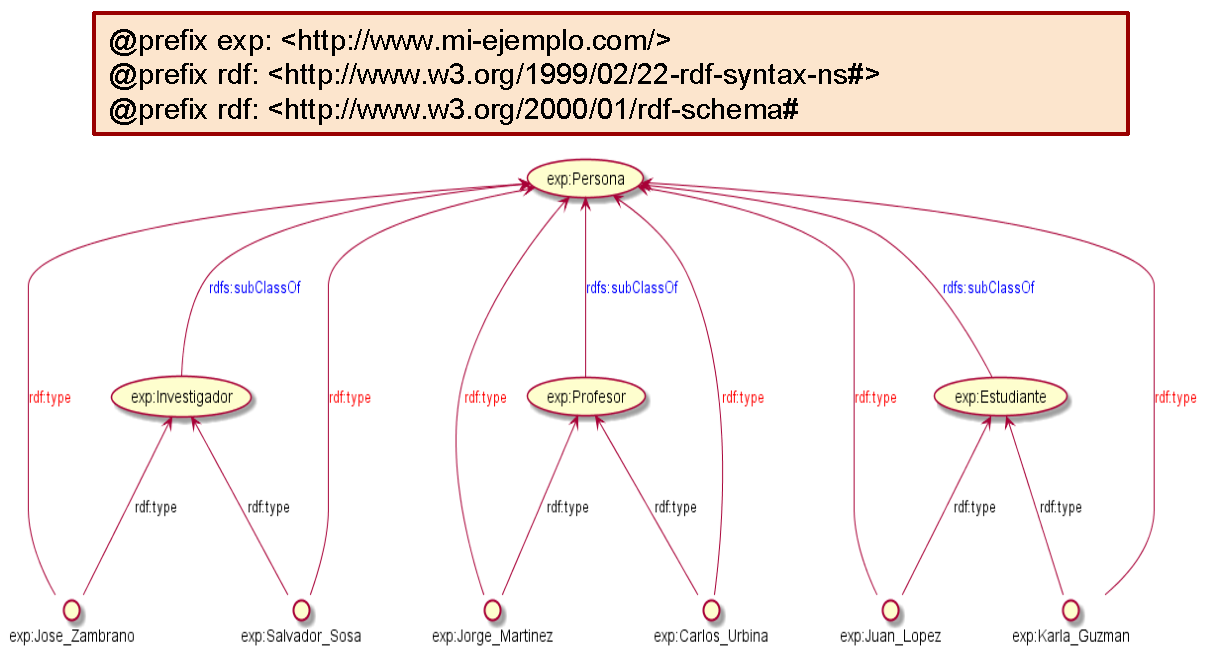
\includegraphics[scale=0.55]{grafoInfBasico} 
	\end{figure}
\end{frame}
%%%%%%%%%%%%%%%%%%%%%%%%%%%%%%%%%%%%%%%%%%%%%%%%%%%%%%%%%%%%%%%%%%%%%%%%%%%%%

\subsubsection{Integraci�n Sem�ntica}
\begin{frame}
	\frametitle{Integraci�n Sem�ntica}
	\begin{block}{Definici�n}
	\justifying
	La b�squeda y recuperaci�n significativa de informaci�n existente en los recursos de informaci�n para responder una consulta dada por un usuario.
	\end{block}
	
	\begin{exampleblock}{Etapas}
	\justifying
	Representar el \textit{conocimiento} de los \textit{recursos de informaci�n} en un \textit{modelo sem�ntico}.
	
	Buscar y recuperar informaci�n existente en la memoria corporativa mediante la interrogaci�n del modelo sem�ntico.
	\end{exampleblock}
\end{frame}
%%%%%%%%%%%%%%%%%%%%%%%%%%%%%%%%%%%%%%%%%%%%%%%%%%%%%%%%%%%%%%%%%%%%%%%%%%%%%%

%%%%%%%%%%%%%%%%%%%%%%%%%%%%%%%%%%%%%%%%%%%%%%%%%%%%%%%%%%%%%%%%%%%%%%%%%%%%%%
\subsection{Descripci�n del Problema}
\subsubsection{Pregunta Investigaci�n}
\begin{frame}
	\frametitle{Pregunta Investigaci�n} 
	\begin{exampleblock}{}
	\justifying 
	\textit{�Las \textbf{tecnolog�as sem�nticas} son viables para solucionar la \textbf{integraci�n sem�ntica} de los \textbf{recursos de informaci�n} de una \textbf{memoria corporativa}?}
	\end{exampleblock}
	
	\begin{figure}
	
\includegraphics[scale=0.4]{PreguntaInv} 
	\end{figure}
\end{frame}

\subsubsection{Objetivos}
\begin{frame}
	\frametitle{Objetivos} 
	\begin{alertblock}{Objetivo Principal}
	\justifying 
	Contribuir a la integraci�n sem�ntica de los recursos de informaci�n en una memoria corporativa, mediante el uso de las tecnolog�as sem�nticas.
	\end{alertblock}
	
	\begin{block}{Objetivos Particulares}
	\begin{enumerate}
	\item \justifying Desarrollar una \textbf{\textit{marco de referencia}} para la \textit{integraci�n sem�ntica} de los \textit{recursos de informaci�n} existentes en una \textit{memoria corporativa}.
	\item \justifying Implementar un \textbf{\textit{modelo sem�ntico}} que representa el \textit{conocimiento expl�cito e impl�cito} de los \textit{recursos de informaci�n}.
	\item \justifying Implementar un \textbf{\textit{prototipo de interfaz gr�fica de usuario}} que permita a los usuarios una interacci�n amigable para la integraci�n sem�ntica de los recursos de informaci�n.
	\item \justifying Evaluar los \textbf{\textit{resultados devueltos}} y \textbf{\textit{tiempos de procesamiento}} en la \textit{integraci�n sem�ntica} para el dominio de redes y telecomunicaciones.
	\end{enumerate}
	\end{block}
\end{frame}

\subsubsection{Metodolog�a}
\begin{frame}
	\frametitle{Metodolog�a}
	\begin{block}{Marco de Referencia}
	\begin{enumerate}
	\item \justifying  Identificar los \textit{casos de uso} para encontrar los principales \textit{recursos de informaci�n} existentes en la memoria, as� como los criterios de b�squeda asociados a �stos.
	\item \justifying  Construir el diagrama de casos de uso.
	\item \justifying  Evaluar herramientas sem�nticas para: edici�n de descripciones sem�nticas, edici�n de reglas de inferencia, gesti�n de modelos sem�nticos.
	\item \justifying  Recopilar los recursos de informaci�n de acuerdo a los casos de uso.
	\item \justifying  Adquirir el conocimiento o informaci�n de los recursos de informaci�n con base en las caracter�sticas y relaciones de los mismos.
	\item \justifying  Construir el diagrama de clases.
	\end{enumerate}
	\end{block}
\end{frame}

\begin{frame}
	\frametitle{Metodolog�a}
	\begin{block}{Marco de Referencia}
	
	\begin{exampleblock}{Modelo Sem�ntico}
	\begin{enumerate}
	\setcounter{enumi}{6}
	\item \justifying  Describir el conocimiento expl�cito de los \textit{recursos de informaci�n} recopilados en un modelo sem�ntico.
	\item \justifying  Identificar las reglas de inferencia a introducir en el modelo, con base en el diagrama de clases.
	\item \justifying  Escribir las reglas de inferencia para enriquecer el modelo sem�ntico con conocimiento impl�cito, mediante el uso del editor de reglas de inferencia.
	\end{enumerate}
	\end{exampleblock}
	
	\begin{enumerate}
	\setcounter{enumi}{9}
	\item \justifying  Identificar las preguntas en lenguaje natural a partir de los casos de uso. \label{item:preguntas}
	\item \justifying  Dise�ar las consultas en el \textit{lenguaje est�ndar de b�squeda} que correspondan a las preguntas en lenguaje natural.
	\end{enumerate}
	\end{block}
\end{frame}

\begin{frame}
	\frametitle{Metodolog�a}
	\begin{block}{Marco de Referencia}	
	\begin{enumerate}
	\setcounter{enumi}{11}
	\item \justifying  Emplear un proceso que permita hacer expl�cito el conocimiento impl�cito.
	\item \justifying  Buscar y recuperar informaci�n en la memoria corporativa, interrogando el modelo sem�ntico.
	\end{enumerate}
	\end{block}
	
	\begin{block}{Prototipo de interfaz gr�fica de usuario}	
	\begin{enumerate}
	\setcounter{enumi}{13}
	\item \justifying  Dise�ar un prototipo para interacci�n (b�squeda y navegaci�n) amigable y trasparente de los usuarios de la memoria con el modelo sem�ntico.
	\item \justifying  Proponer funcionalidades b�sicas del prototipo.
	\item \justifying  Indicar cu�les son las interfaces para los usuarios (pantallas).
	\item \justifying  Describir las especificaciones de estas interfaces.
	\item \justifying  Implementar el prototipo y realizar pruebas del mismo.
	\end{enumerate}
	\end{block}
\end{frame}

\begin{frame}
	\frametitle{Metodolog�a}
	\begin{block}{Evaluar los resultados devueltos}
	\begin{enumerate}
	\setcounter{enumi}{18}
	\item \justifying  Evaluar la calidad de los resultados (recursos relevantes recuperados) con y sin inferencia, mediante el uso de m�tricas que se emplean en la recuperaci�n de la informaci�n: exhaustividad y precisi�n.
	\item \justifying  Identificar aquellos recursos (total de recursos relevantes) que responden las preguntas del paso \ref{item:preguntas} de este listado. \label{item:identrec}
	\item \justifying  Consultar al modelo sem�ntico y comparar los recursos relevantes recuperados con los recursos relevantes que se identificaron en el paso \ref{item:identrec} de este listado.
	\item \justifying  Calcular la exhaustividad y precisi�n.
	\end{enumerate}
	\end{block}
\end{frame}

\begin{frame}
	\frametitle{Metodolog�a}
	\begin{block}{Evaluar los tiempos de procesamiento}
	\begin{enumerate}
	\setcounter{enumi}{22}
	\item \justifying  Evaluar los \textit{tiempos promedios} que toma la herramienta electa de gesti�n de los modelos sem�nticos, para consultar los modelos con/sin inferencia.
	\item \justifying  Elaborar un script que calcule `\textbf{\textit{n}}' veces el \textit{tiempo de procesamiento} al consultar un modelo sem�ntico (con o sin inferencia). Las consultas se hacen a las preguntas identificadas del paso \ref{item:preguntas} de este listado.
	\end{enumerate}
	\end{block}
\end{frame}

\subsubsection{Hip�tesis}
\begin{frame}
	\frametitle{Hip�tesis}
	\begin{block}{}
	\justifying 
	\textbf{El uso de las \textit{tecnolog�as sem�nticas} es adecuado para lograr la \textit{integraci�n sem�ntica} de \textit{recursos de informaci�n} en una \textit{memoria corporativa}}.
	\end{block}
	
	\begin{figure}
	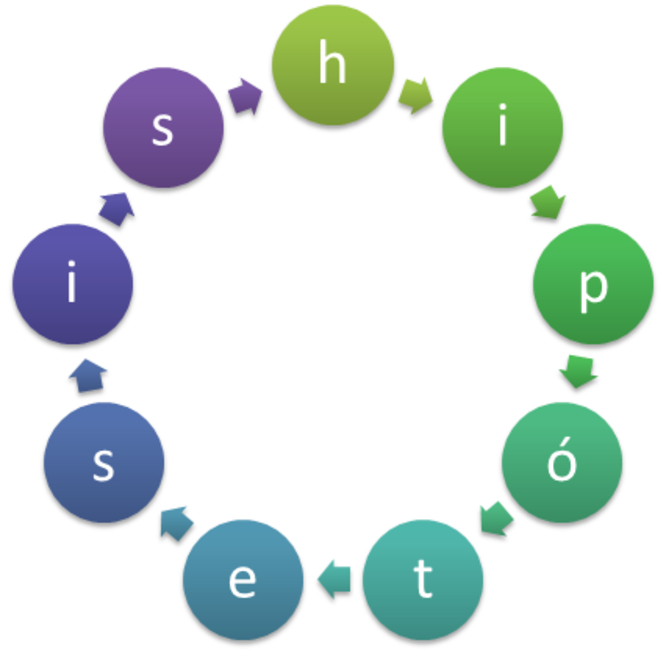
\includegraphics[scale=0.49]{hipotesis} 
	\end{figure}
\end{frame}

\subsubsection{Aportaciones}
\begin{frame}
	\frametitle{Aportaciones}
	\begin{enumerate}
	\item \justifying Un \textit{marco de referencia} para lograr la integraci�n sem�ntica de recursos de informaci�n.
    \item \justifying Un modelo sem�ntico que representa el conocimiento de una memoria corporativa, el cual tiene tres ramas principales (Personas, Recursos Digitales y Conceptos del Redes y Telecomunicaciones).
    \item \justifying  Un prototipo (interfaz gr�fica de usuario) para la interacci�n amigable (b�squeda y consulta de informaci�n) de los usuarios al modelo sem�ntico.
    \item \justifying Los resultados de nuestra evaluaci�n experimental.
    \item \justifying Un par de scripts para la generaci�n autom�tica y controlada de descripciones (conocimiento expl�cito) de los \textit{recursos de informaci�n}, con el fin de poblar la base de conocimiento.
	\end{enumerate}
\end{frame}
%%%%%%%%%%%%%%%%%%%%%%%%%%%%%%%%%%%%%%%%%%%%%%%%%%%%%%%%%%%%%%%%%%%%%%%%%%%%%%
\section{Integraci�n Sem�ntica de una Memoria Corporativa}
%%%%%%%%%%%%%%%%%%%%%%%%%%%%%%%%%%%%%%%%%%%%%%%%%%%%%%%%%%%%%%%%%%%%%%%%%%%%%%
\begin{frame}
	\frametitle{Marco de Referencia}
	\begin{block}{Etapas}
		\begin{enumerate}
		\item \justifying Representar las caracter�sticas y/o relaciones de los \textit{recursos de informaci�n} mediante el est�ndar RDF, para construir un modelo sem�ntico.
		\item \justifying Introducir \textit{reglas de inferencia} en el modelo sem�ntico, para enriquecer con \textit{conocimiento impl�cito} de los \textit{recursos de informaci�n} y del dominio de la memoria.
		\item \justifying Buscar y recuperar informaci�n en el modelo sem�ntico para responder un conjunto consultas SPARQL.
		\end{enumerate}
	\end{block}
\end{frame}
%%%%%%%%%%%%%%%%%%%%%%%%%%%%%%%%%%%%%%%%%%%%%%%%%%%%%%%%%%%%%%%%%%%%%%%%%%%%%%

%%%%%%%%%%%%%%%%%%%%%%%%%%%%%%%%%%%%%%%%%%%%%%%%%%%%%%%%%%%%%%%%%%%%%%%%%%%%%%
\begin{frame}
	\frametitle{Arquitectura de la Integraci�n Sem�ntica}	
	\begin{figure}
	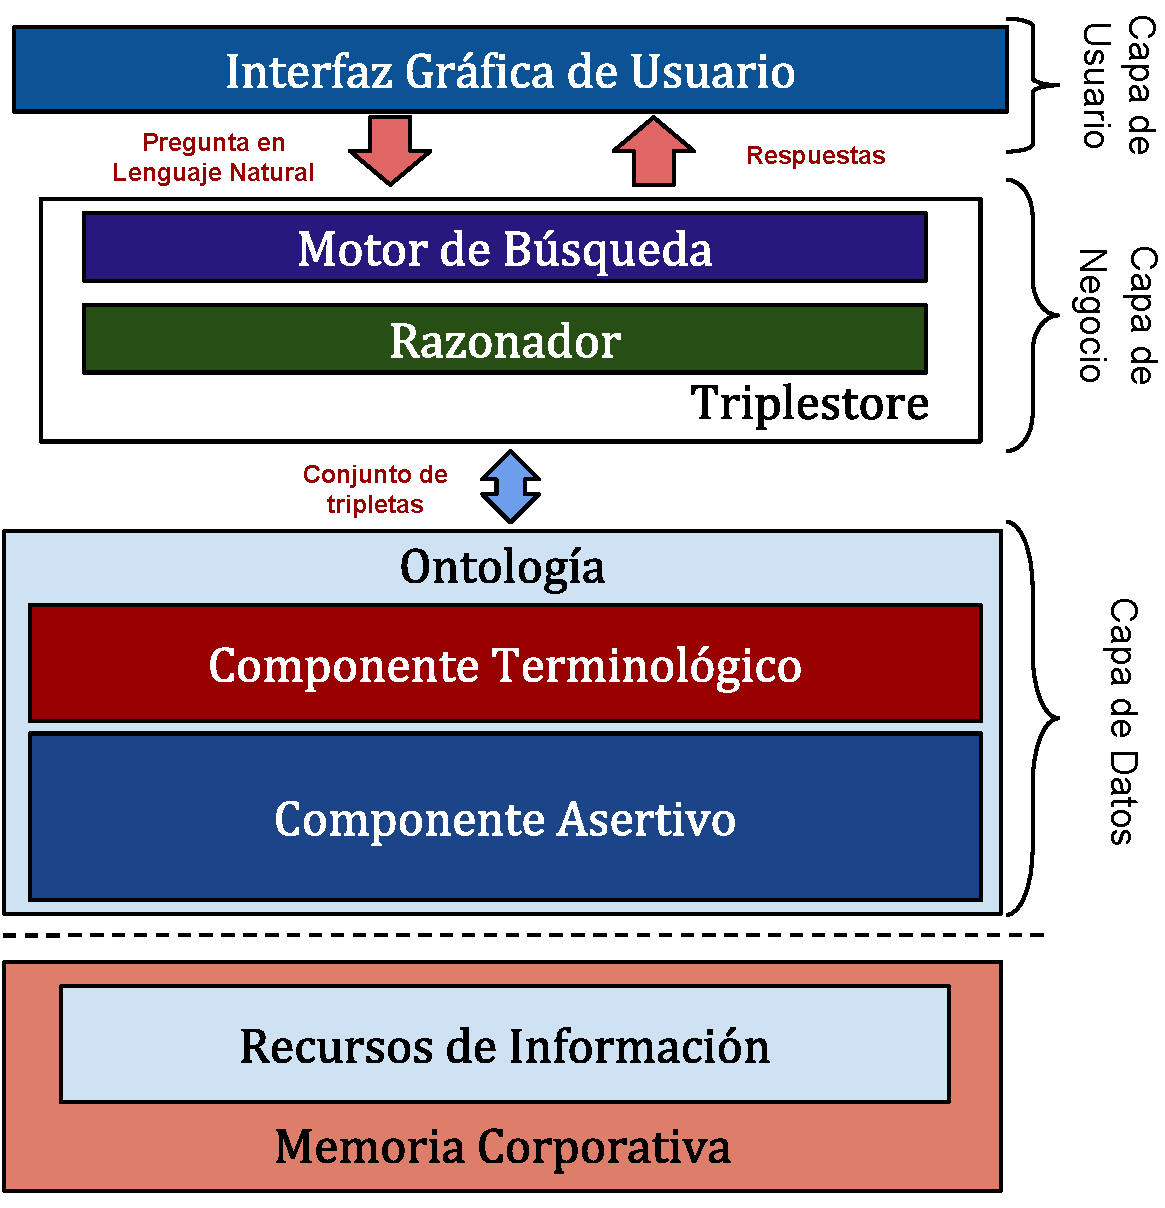
\includegraphics[scale=0.33]{Arquitectura} 
	\end{figure}
\end{frame}
%%%%%%%%%%%%%%%%%%%%%%%%%%%%%%%%%%%%%%%%%%%%%%%%%%%%%%%%%%%%%%%%%%%%%%%%%%%%%%

%%%%%%%%%%%%%%%%%%%%%%%%%%%%%%%%%%%%%%%%%%%%%%%%%%%%%%%%%%%%%%%%%%%%%%%%%%%%%%
\begin{frame}
	\frametitle{Casos de Uso}
	
	\begin{block}{}
		\begin{itemize}
		\item \justifying \textbf{\textit{Cartograf�a de Competencias}} es la b�squeda y recuperaci�n de informaci�n significativa de las personas a partir de las caracter�sticas personales y profesionales de las mismas.
		\item \justifying \textbf{\textit{B�squeda de Recursos Digitales}} es la b�squeda y recuperaci�n de informaci�n significativa de los documentos y archivos multimedia a partir del contenido de los mismos.
		\end{itemize}
	\end{block}
	
	\begin{figure}
	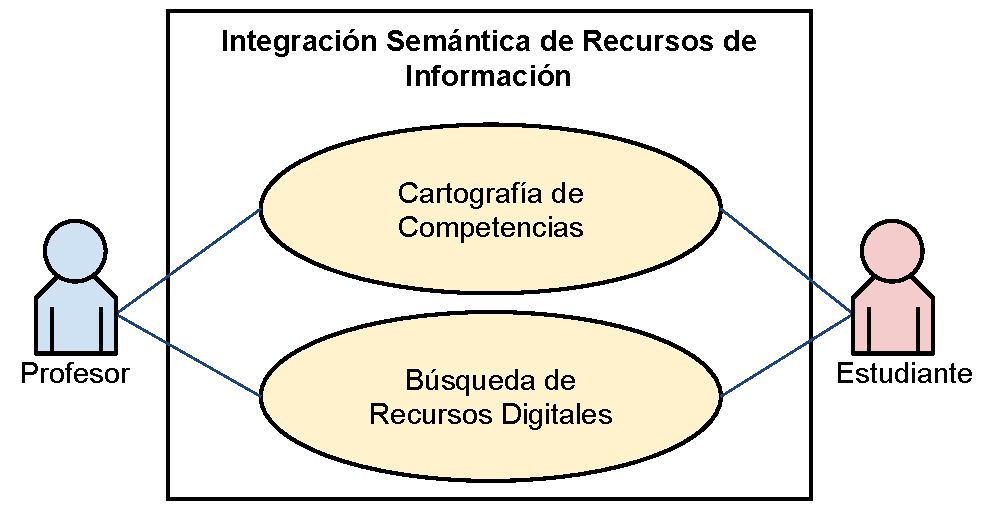
\includegraphics[scale=0.56]{CasosUso} 
	\end{figure}
\end{frame}
%%%%%%%%%%%%%%%%%%%%%%%%%%%%%%%%%%%%%%%%%%%%%%%%%%%%%%%%%%%%%%%%%%%%%%%%%%%%%%

%%%%%%%%%%%%%%%%%%%%%%%%%%%%%%%%%%%%%%%%%%%%%%%%%%%%%%%%%%%%%%%%%%%%%%%%%%%%%%
\subsection{Representaci�n el Conocimiento}
\subsubsection{Identificar los principales recursos de informaci�n}
\begin{frame}
	\frametitle{Identificar los principales recursos de informaci�n}	
	\begin{figure}
	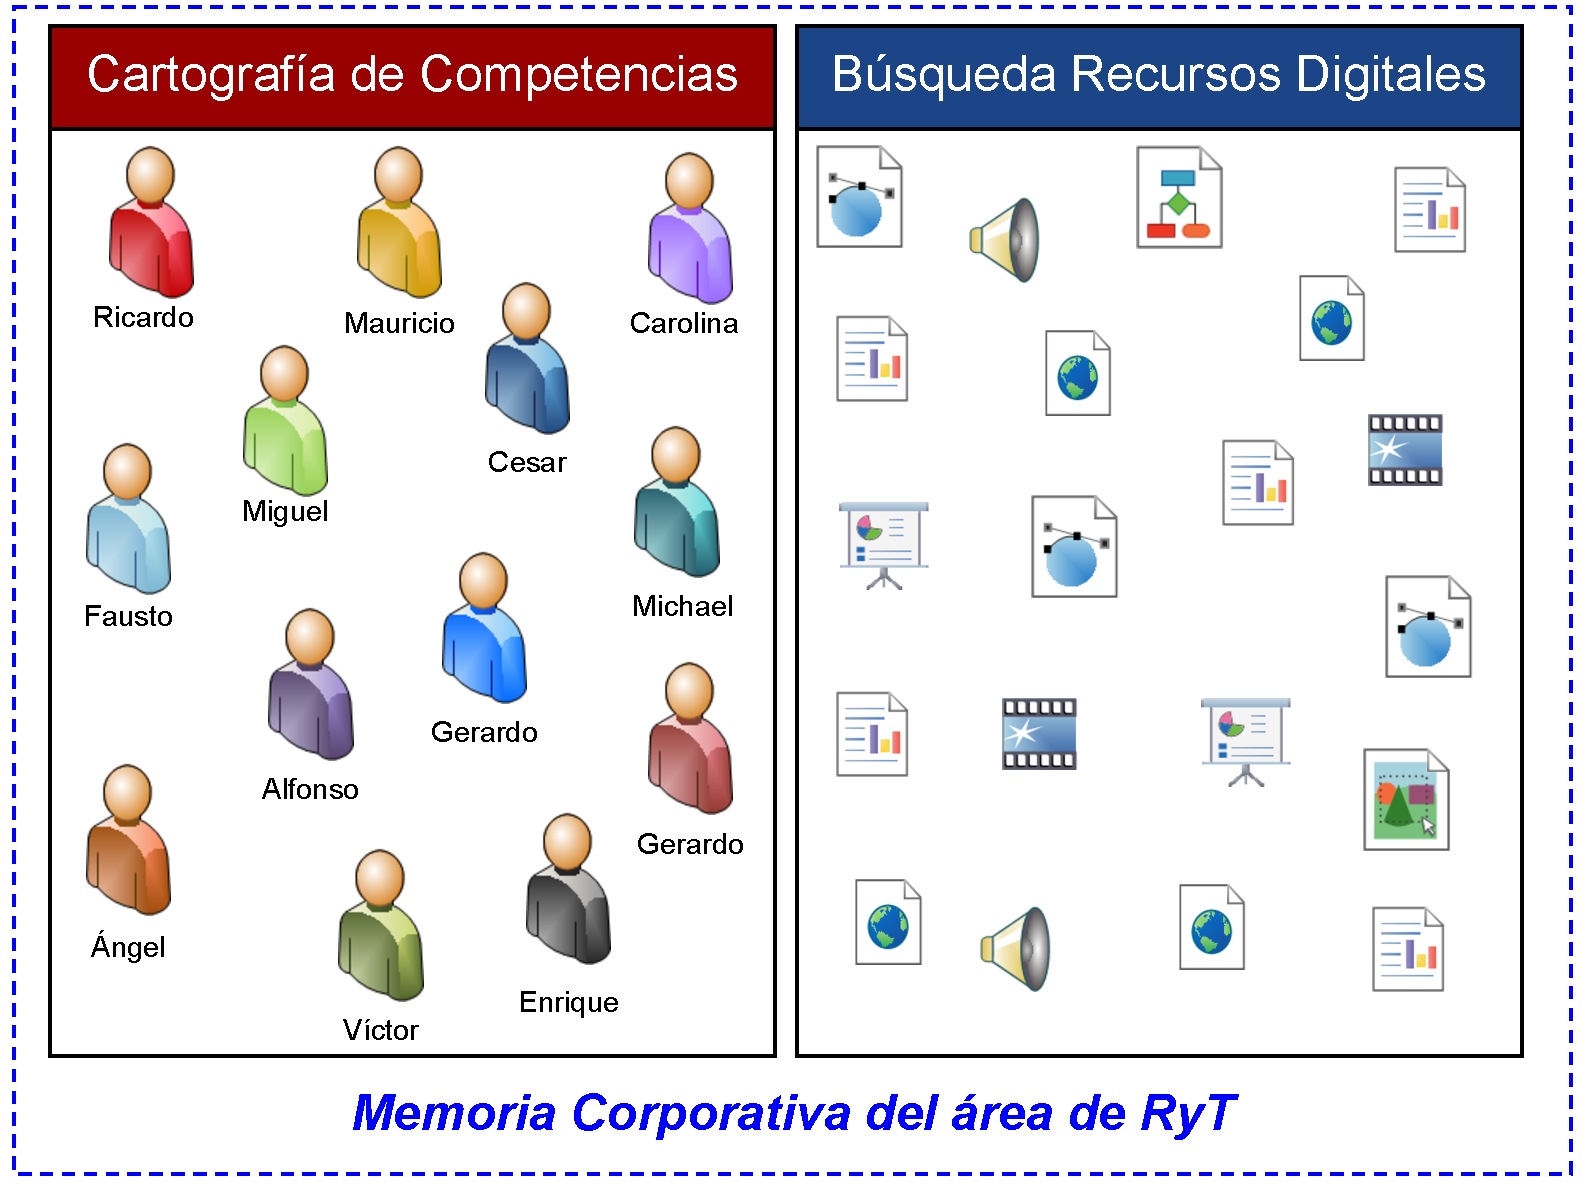
\includegraphics[scale=0.33]{CasosUsoMC} 
	\end{figure}
\end{frame}

\subsubsection{Adquirir y expresar el conocimiento de los recursos de informaci�n}
\begin{frame}
	\frametitle{Adquirir y expresar el conocimiento de los recursos de informaci�n}	
	\begin{figure}
	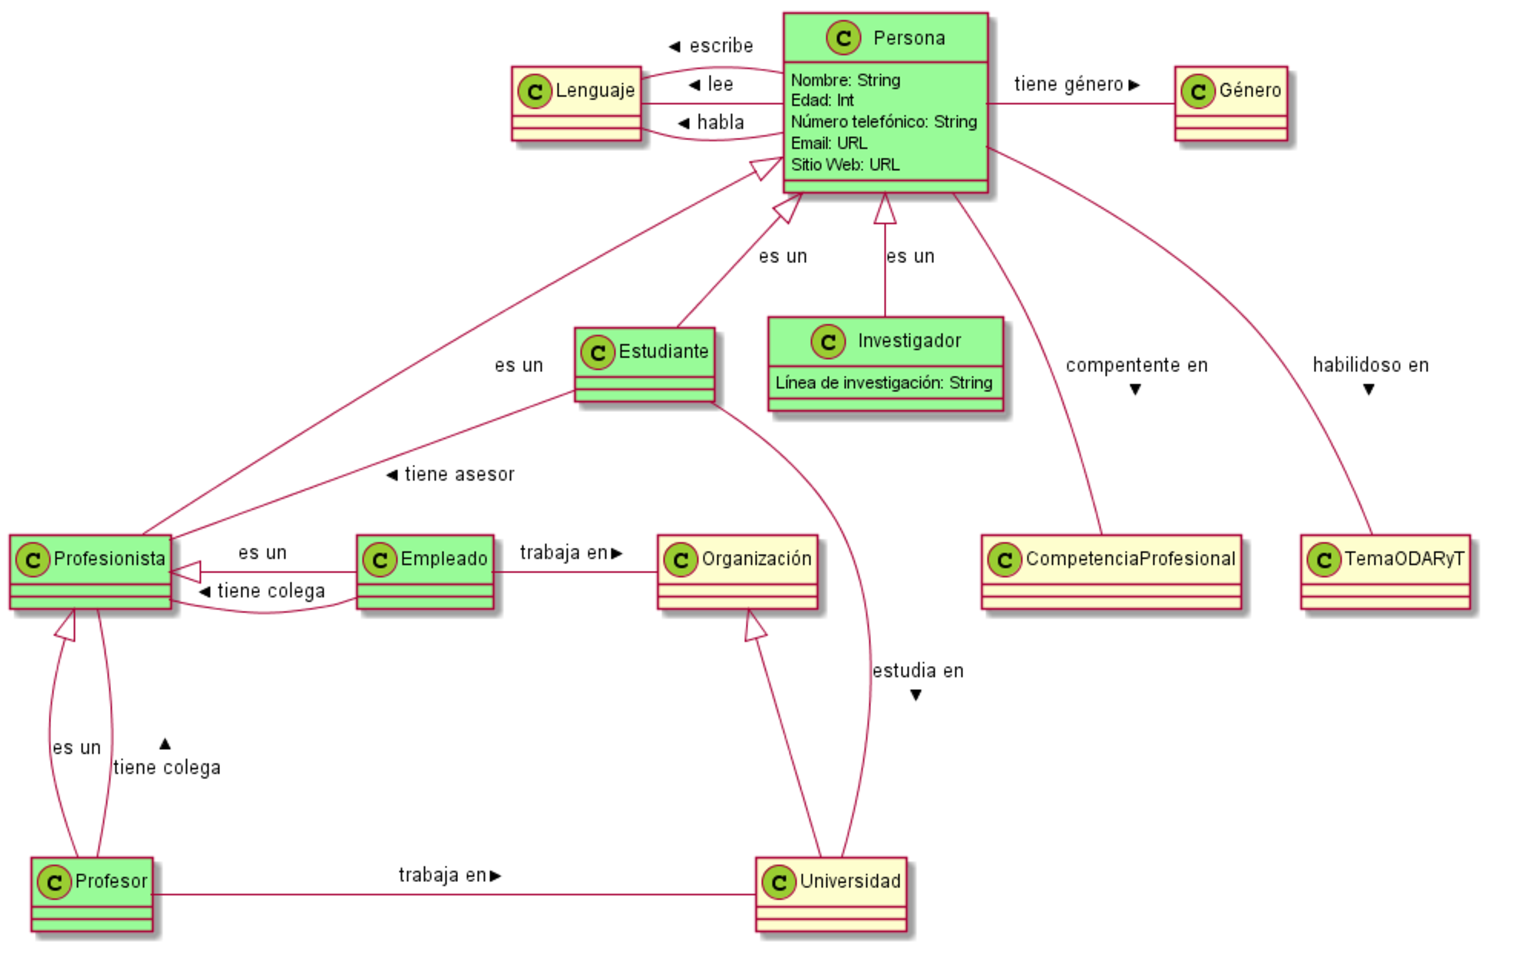
\includegraphics[scale=0.38]{CasoUsoCartComp} 
	\end{figure}
\end{frame}

\subsubsection{Representar el conocimiento e informaci�n mediante el est�ndar RDF}
\begin{frame}
	\frametitle{Representar el conocimiento e informaci�n mediante el est�ndar RDF}
	
	\begin{block}{Definici�n}
	\justifying 
	Marco gen�rico para describir el conocimiento e informaci�n expl�cita de los recursos mediante sus caracter�sticas y relaciones. \begin{scriptsize}\cite{SurvSemWeb2012}\end{scriptsize}
	\end{block}
	
	\begin{block}{Actividades en la representaci�n del conocimiento}
	\begin{enumerate}
	\item \justifying Asignar un \textit{identificador �nico de recursos} (URI) a cada \textit{recurso de informaci�n} en la \textit{memoria corporativa}.
	\item \justifying Asignar un URI a cada caracter�stica y/o relaci�n (propiedad) de de los \textit{recursos de informaci�n}.
	\item \justifying Generar las tripletas RDF asociadas a las descripciones de los recursos de informaci�n.
	\end{enumerate}
	\end{block}
%	\begin{figure}
%	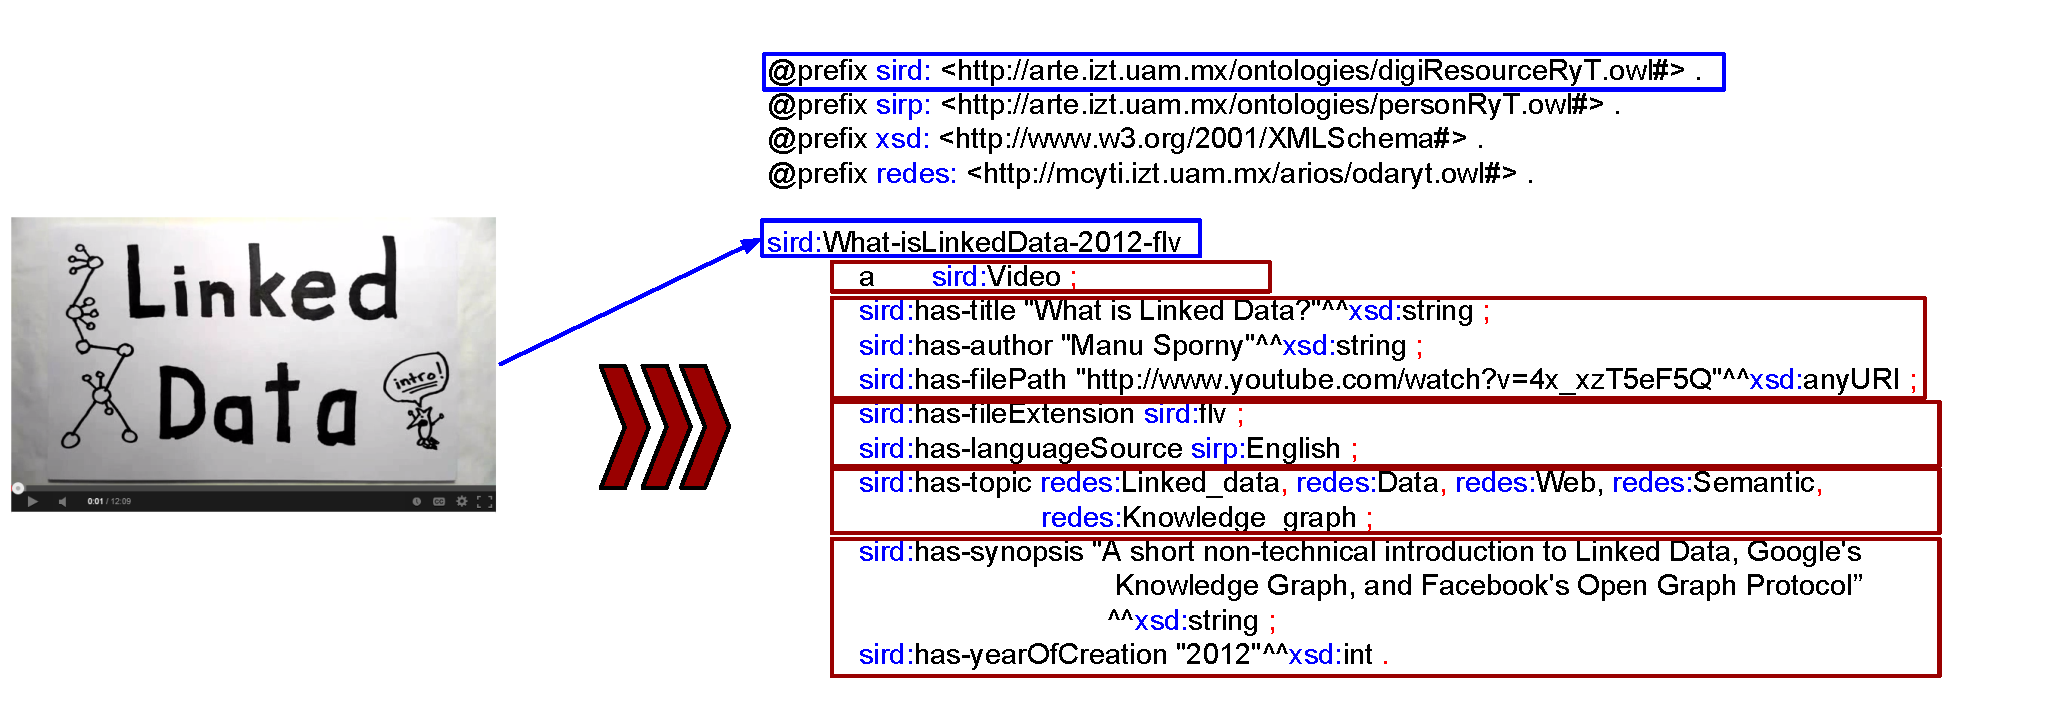
\includegraphics[scale=0.38]{Vid2RDF}
%	\end{figure}
	%%%%%%%%%%%%%%%%%%%%%%%
\end{frame}

\begin{frame}
	\frametitle{Representar el conocimiento e informaci�n mediante el est�ndar RDF}
	\begin{figure}
	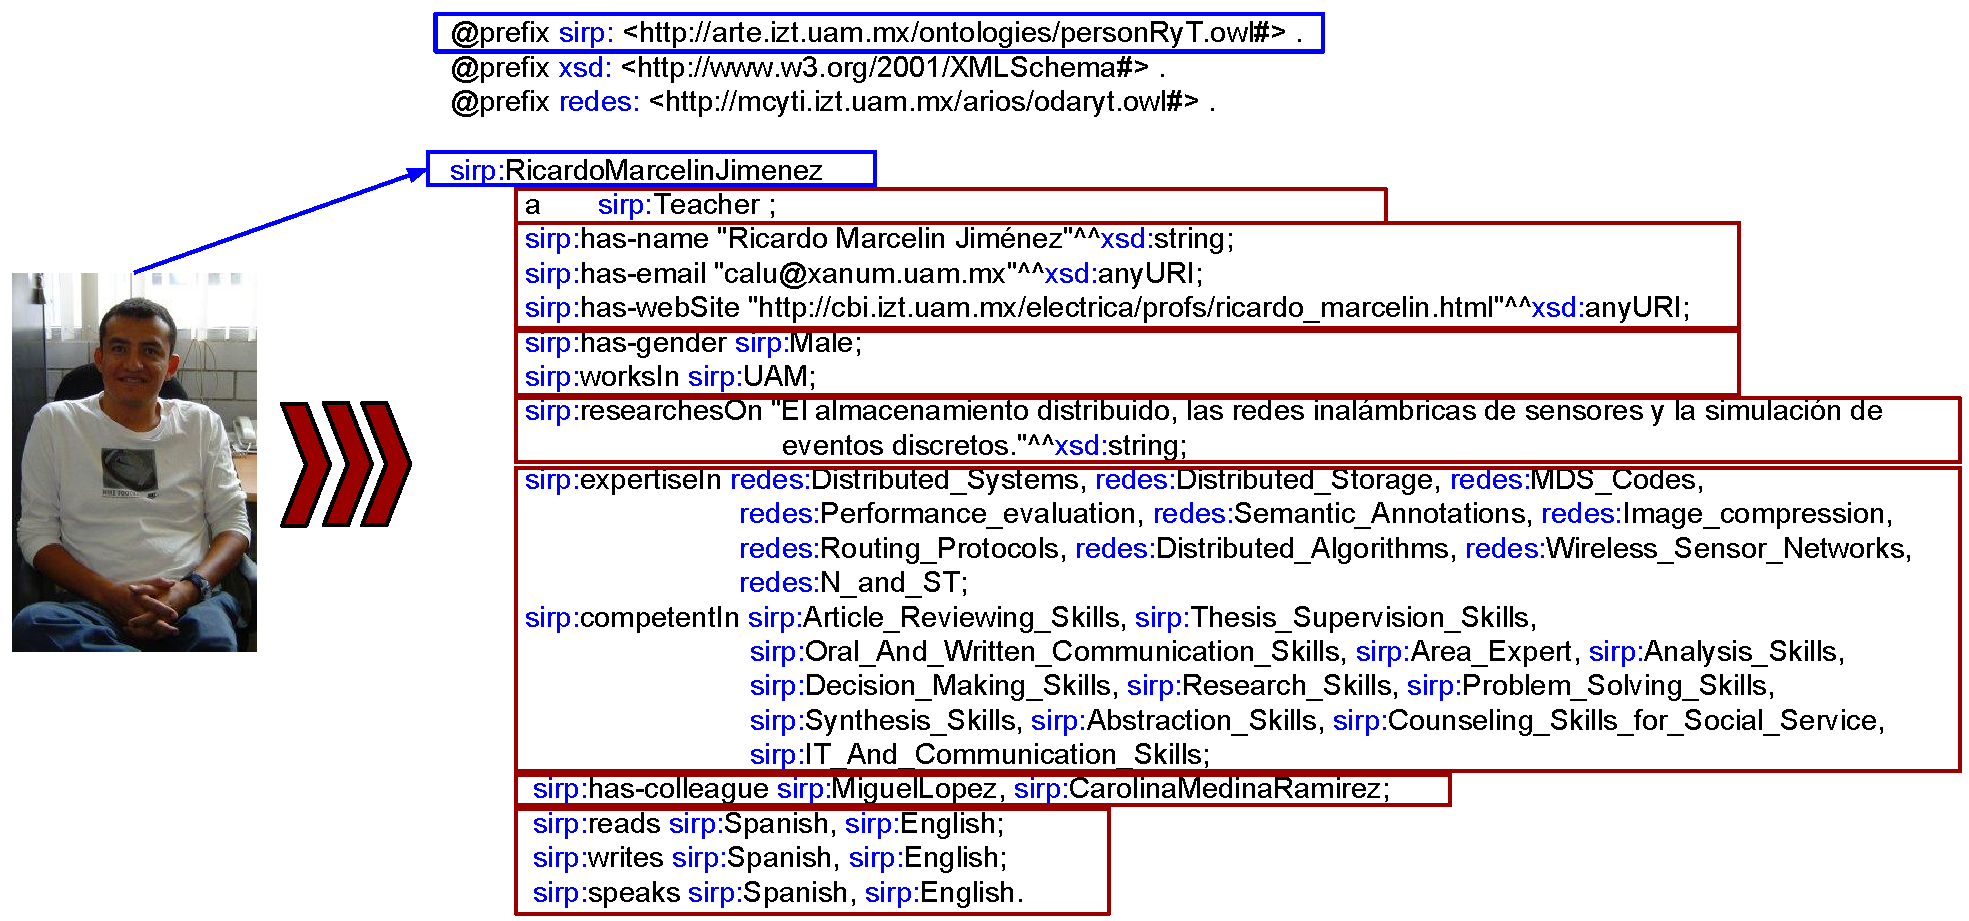
\includegraphics[scale=0.35]{Person2RDF}
	\end{figure}
\end{frame} 

\begin{frame}
	\frametitle{Representar el conocimiento e informaci�n mediante el est�ndar RDF}
	\begin{figure}
	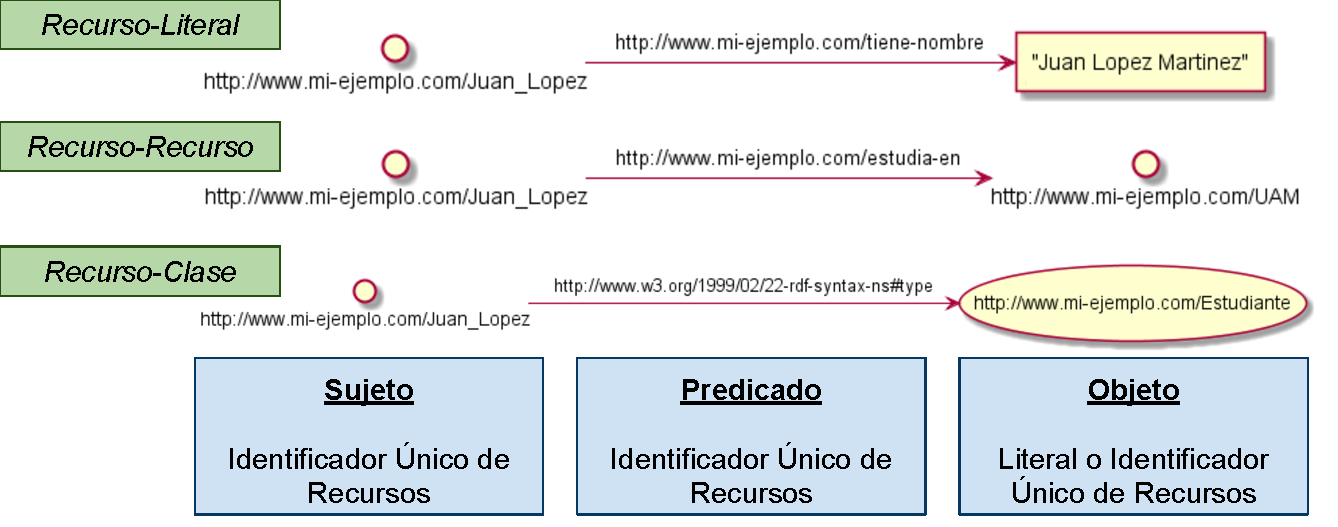
\includegraphics[scale=0.45]{Tripletas} 
	\end{figure}
\end{frame}

\begin{frame}
	\frametitle{Representar el conocimiento e informaci�n mediante el est�ndar RDF}
	\begin{figure}
	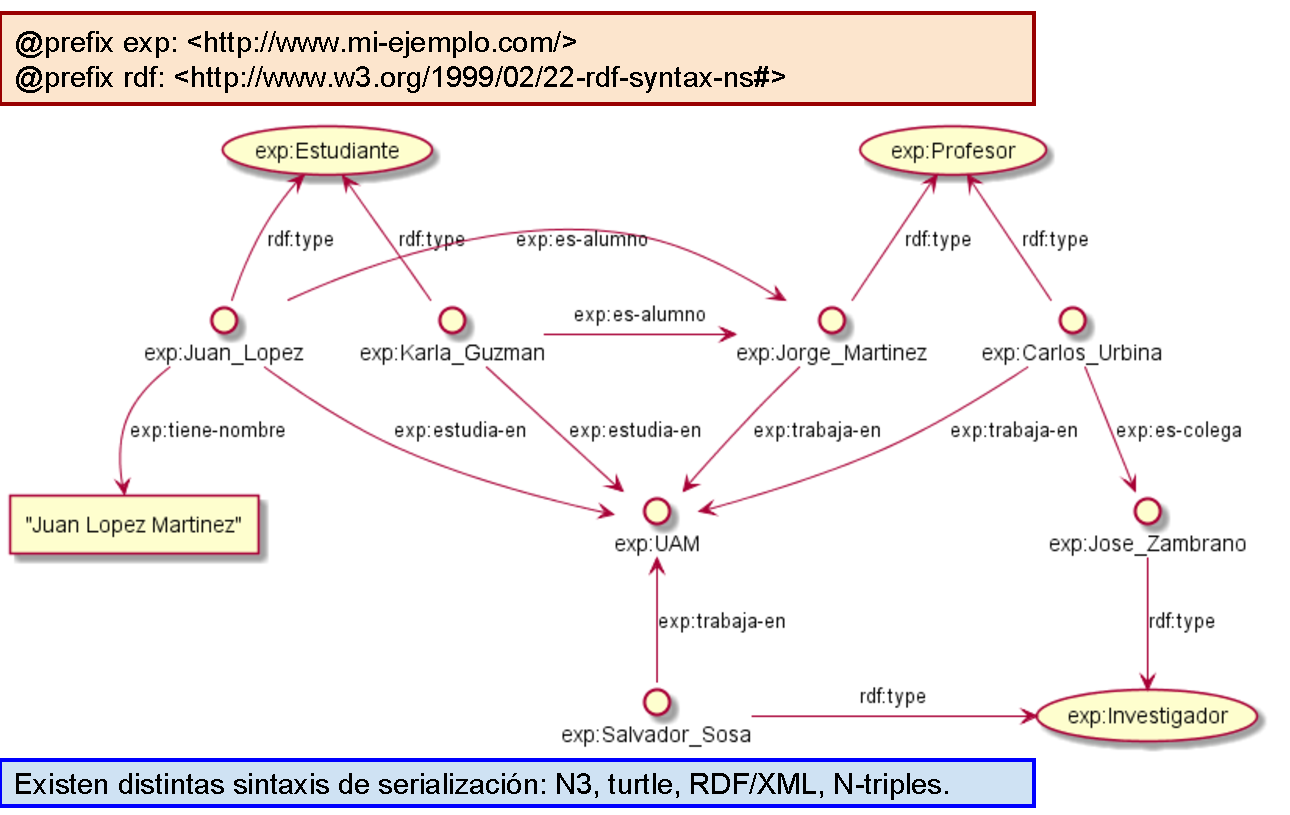
\includegraphics[scale=0.48]{GrafoRDF} 
	\end{figure}
\end{frame}

%%%%%%%%%%%%%%%%%%%%%%%%%%%%%%%%%%%%%%%%%%%%%%%%%%%%%%%%%%%%%%%%%%%%%%%%%%%%%%

\subsection{Enriquecer el conocimiento en el modelo sem�ntico}
\begin{frame}
	\frametitle{Ontolog�a}
	%%%%%%%%%%%%%%%%%%%%%%%%%%%%
	\begin{alertblock}{Definici�n}
	\justifying 
	Una definici�n formal, expl�cita y compartida de los conceptos, as� como las relaciones de un determinado dominio. \begin{scriptsize}\cite{Gruber}\end{scriptsize}
	\end{alertblock}
	
	\begin{block}{Componentes}
	\begin{itemize}
	\item \justifying \textbf{\textit{Componente Asertivo (ABox)}} est� constituido por descripciones que afirman que los individuos son instancias de una clase o propiedad.
	\item \justifying \textbf{\textit{Componente Terminol�gico (TBox)}} describe las clases y propiedades relevantes, as� como las reglas de inferencia que permiten aprovechar la manera en que las instancias se relacionan entre s�.
	\end{itemize}
	\end{block}
	%%%%%%%%%%%%%%%%%%%%%%%%%%%%
\end{frame}

\begin{frame}
	\frametitle{Axiomatizaci�n}	
	\begin{block}{Reglas de inferencia o Axiomas}
	\justifying 
	Expresiones para enriquecer un grafo RDF con conocimiento impl�cito.\\
	\end{block}
	
	\begin{block}{Lenguajes}
	Especificaciones para describir clases, propiedades e individuos.
	\begin{itemize}
	\item \justifying \textit{RDF Schema \textbf{RDF(S)}}
	\item \justifying \textit{Web Ontology Language \textbf{OWL}} 
	\end{itemize}
	\end{block}
	
	\begin{figure}
	
\includegraphics[scale=0.4]{PrefijosRDFSOWL}
	\end{figure}
	
	\begin{block}
	\justifying
	\textit{Lo que es obvio para un humano, no lo es para una maquina}.
	\end{block}
\end{frame}

%\begin{frame}
%	\frametitle{Enriquecer el conocimiento en el modelo sem�ntico}
%	\begin{block}{}
%	\justifying
%	Para cada \textit{caso de uso} debe encontrarse el respectivo conjunto de axiomas (TBox).
%	\end{block}
%	
%	\begin{figure}
%	
\includegraphics[scale=0.4]{PrefijosRDFSOWL}
%	\end{figure}
%\end{frame}
	
\subsubsection{Herencia de Clases}
\begin{frame}[allowframebreaks]
	\frametitle{Herencia de Clases}
	\begin{block}{Subclase (rdfs:subClassOf)}
	\justifying
	Afirma que una \textit{clase A} se subsume por una \textit{clase B}, es decir, la clase A es un caso particular de la \textit{clase B}. En este caso, las instancias de la clase A son instancias de la clase B.
	\end{block}
	
	\begin{figure}
	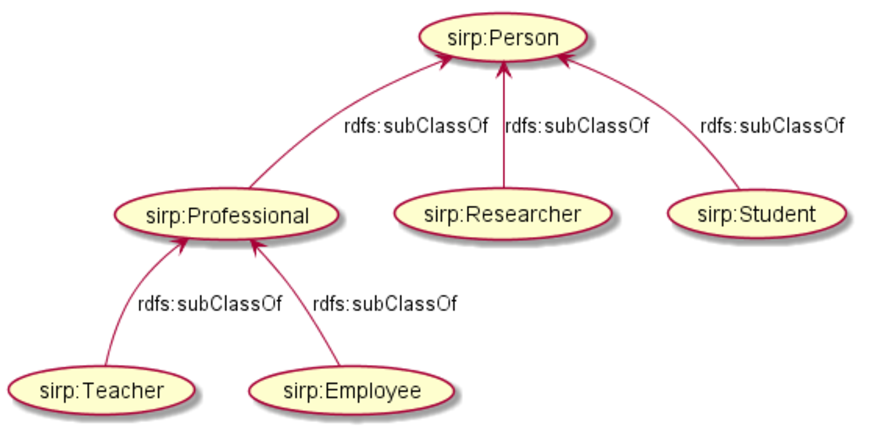
\includegraphics[scale=0.5]{HerenClassCartComp}
	\end{figure}
	%%%%%%%%%%%%%%%%%%%%%%%
	
	\begin{figure}
	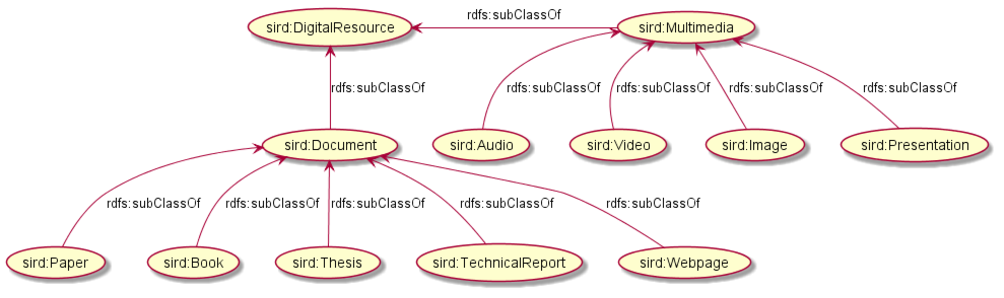
\includegraphics[scale=0.68]{HerenClassRecDigi}
	\end{figure}
	%%%%%%%%%%%%%%%%%%%%%%%
	
	\begin{figure}
	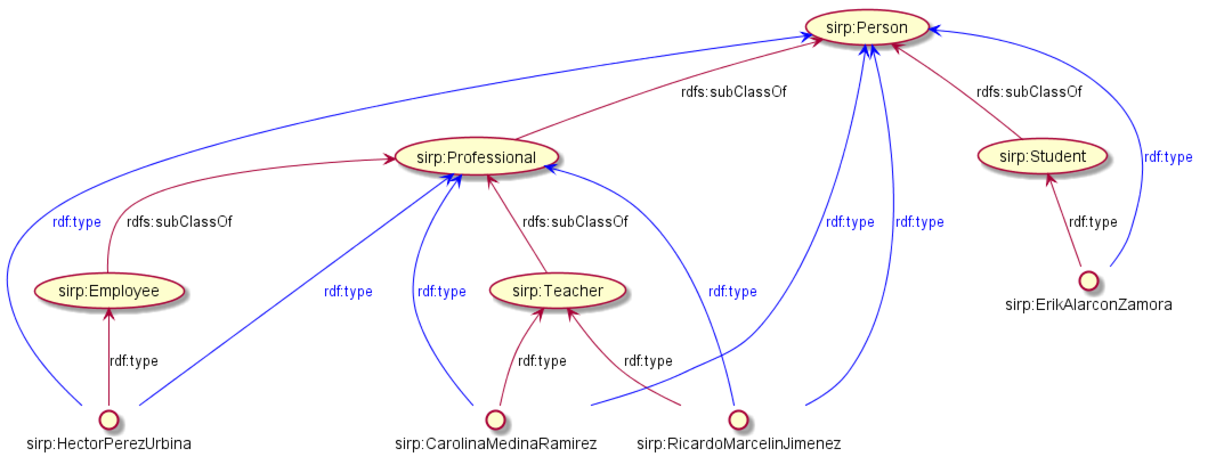
\includegraphics[scale=0.57]{EjmpInfSubClass}
	\end{figure}
	%%%%%%%%%%%%%%%%%%%%%%%
\end{frame}

\subsubsection{Herencia de Propiedades}
\begin{frame}[allowframebreaks]
	\frametitle{Herencia de Propiedades}
	\begin{block}{Subpropiedad (rdfs:subPropertyOf)}
	\justifying
	Afirma que todos los recursos que se relacionan por la \textit{propiedad X}, tambi�n se relacionan por la \textit{propiedad Y}.
	\end{block}
	
	\begin{figure}
	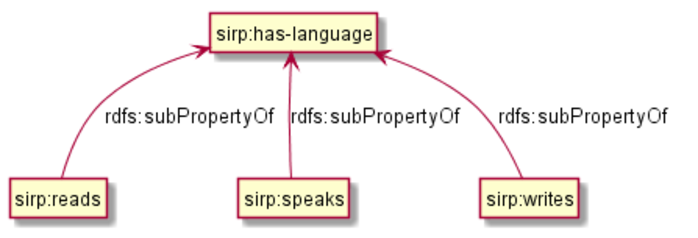
\includegraphics[scale=0.57]{HerPropLang}
	\end{figure}
		
	\begin{figure}
	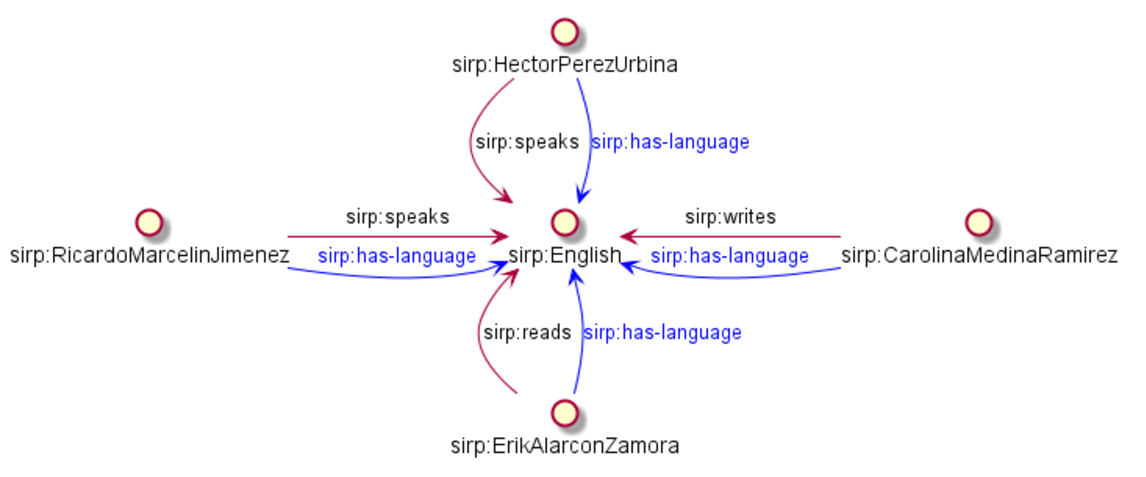
\includegraphics[scale=0.55]{EjmpInfProp}
	\end{figure}
	%%%%%%%%%%%%%%%%%%%%%%%
\end{frame}

\subsubsection{Dominio y Rango en las Propiedades}
\begin{frame}[allowframebreaks]
	\frametitle{Dominio y Rango en las Propiedades}
	\begin{block}{Dominio (rdfs:domain)}
	\justifying
	Especifica qu� clase se aplica a una propiedad.
	\end{block}
	
	\begin{block}{Rango (rdfs:range)}
	\justifying
	Especifica los valores (clase o tipo de literal) que puede asumir una propiedad.
	\end{block}
	
	\begin{figure}
	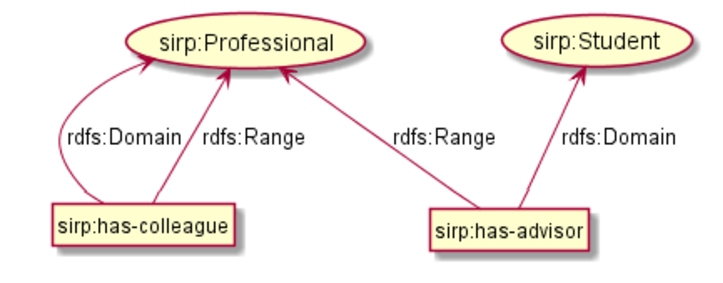
\includegraphics[scale=0.52]{exAxDyRPer}
	\end{figure}
	%%%%%%%%%%%%%%%%%%%%%%%
	
	\begin{figure}
	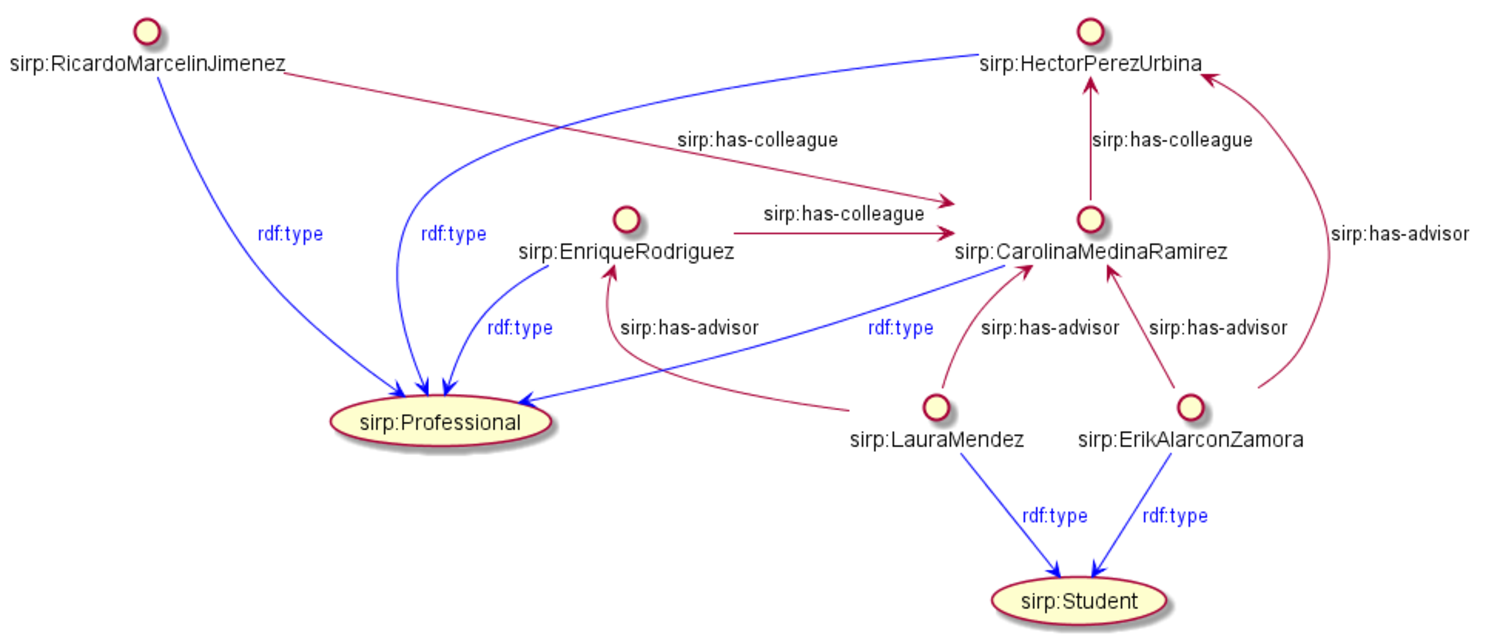
\includegraphics[scale=0.45]{exInfDyRPer}
	\end{figure}
	%%%%%%%%%%%%%%%%%%%%%%%
\end{frame}

\subsubsection{Caracter�sticas en las Propiedades}
\begin{frame}
	\frametitle{Caracter�sticas en las propiedades}
	\begin{block}{Propiedad sim�trica (owl:SymmetricProperty)}
	\justifying
	Afirma que la \textit{propiedad X} es su propia propiedad inversa, es decir, si la \textit{propiedad X} relaciona al \textit{individuo A} con el \textit{individuo B}, entonces, esta propiedad debe relacionar al \textit{individuo B} con el \textit{individuo A}.
	\end{block}
	
	\begin{figure}
	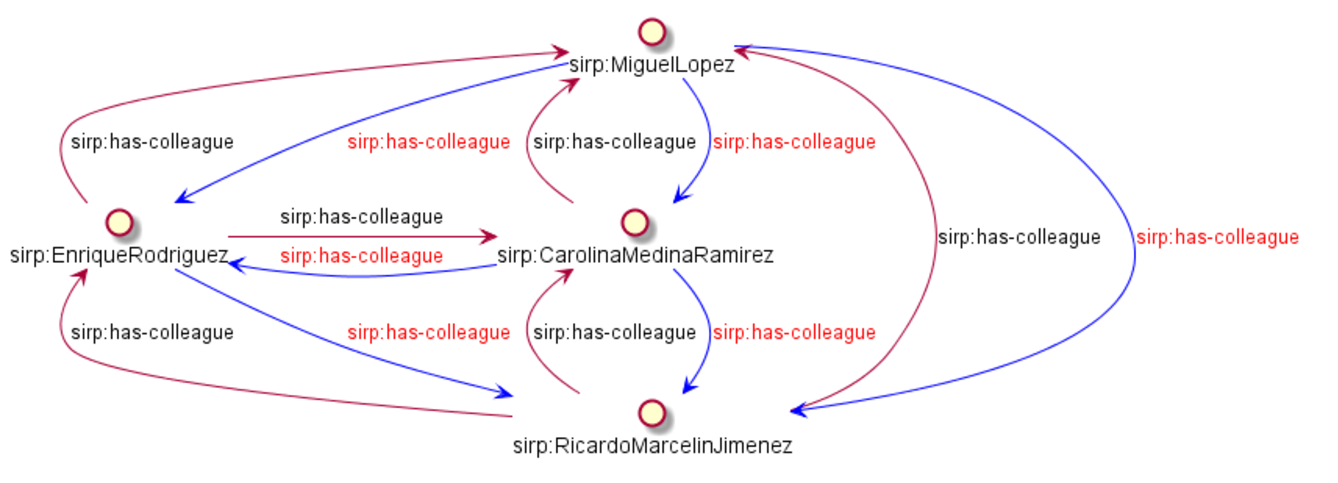
\includegraphics[scale=0.5]{infSymColl}
	\end{figure}
	%%%%%%%%%%%%%%%%%%%%%%%
\end{frame}
%%%%%%%%%%%%%%%%%%%%%%%%%%%%%%%%%%%%%%%%%%%%%%%%%%%%%%%%%%%%%%%%%%%%%%%%%%%%%%

\subsection{Buscar y recuperar la informaci�n en el modelo sem�ntico}
\begin{frame}
	\frametitle{Buscar y recuperar la informaci�n en el modelo sem�ntico}
%	\begin{block}{Objetivo}
%	\justifying
%	La b�squeda y recuperaci�n de la informaci�n para responder las preguntas o necesidades informativas de los usuarios del �rea de Redes y Telecomunicaciones (RyT).
%	\end{block}
	
	\begin{block}{SPARQL}
	\justifying 
	Lenguaje de consulta y protocolo de acceso a RDF, para la b�squeda y recuperaci�n de la informaci�n en un grafo RDF.
	\end{block}
	
	\begin{figure}
	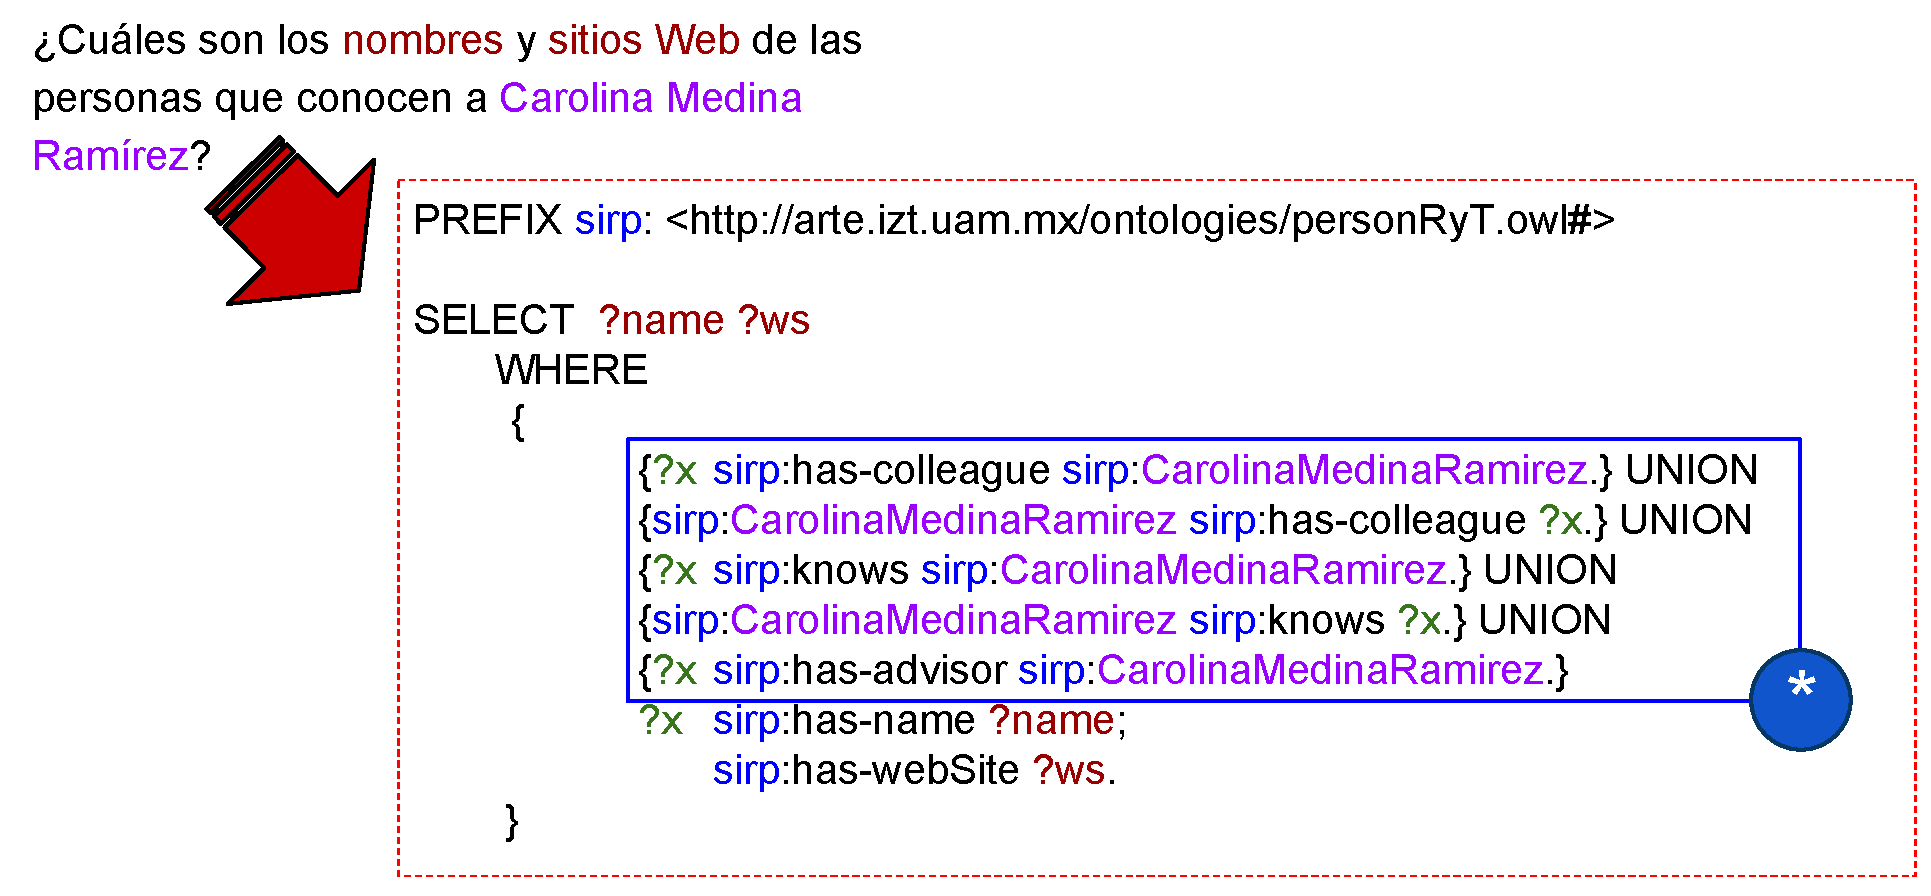
\includegraphics[scale=0.32]{q2rqlSR}
	\end{figure}
	
%	\begin{block}{Actividades}
%	\begin{enumerate}
%	\item \justifying Identificar las preguntas en lenguaje natural.
%	\item \justifying Transformar las preguntas a una consultas SPARQL.
%	\item \justifying Ejecutar las consultas mediante un motor de b�squeda SPARQL.
%	\end{enumerate}
%	\end{block}

\end{frame}

%%%%%%%%%%%%%%%%%%%%%%%%%%%%%%%%%%%%%%%%%%%%%%%%%%%%%%%%%%%%%%%%%%%%%%%%%%%%%%
\subsubsection{B�squeda + Inferencia}
\begin{frame}[allowframebreaks]
	\frametitle{Uso de inferencia}
		
	\begin{figure}
	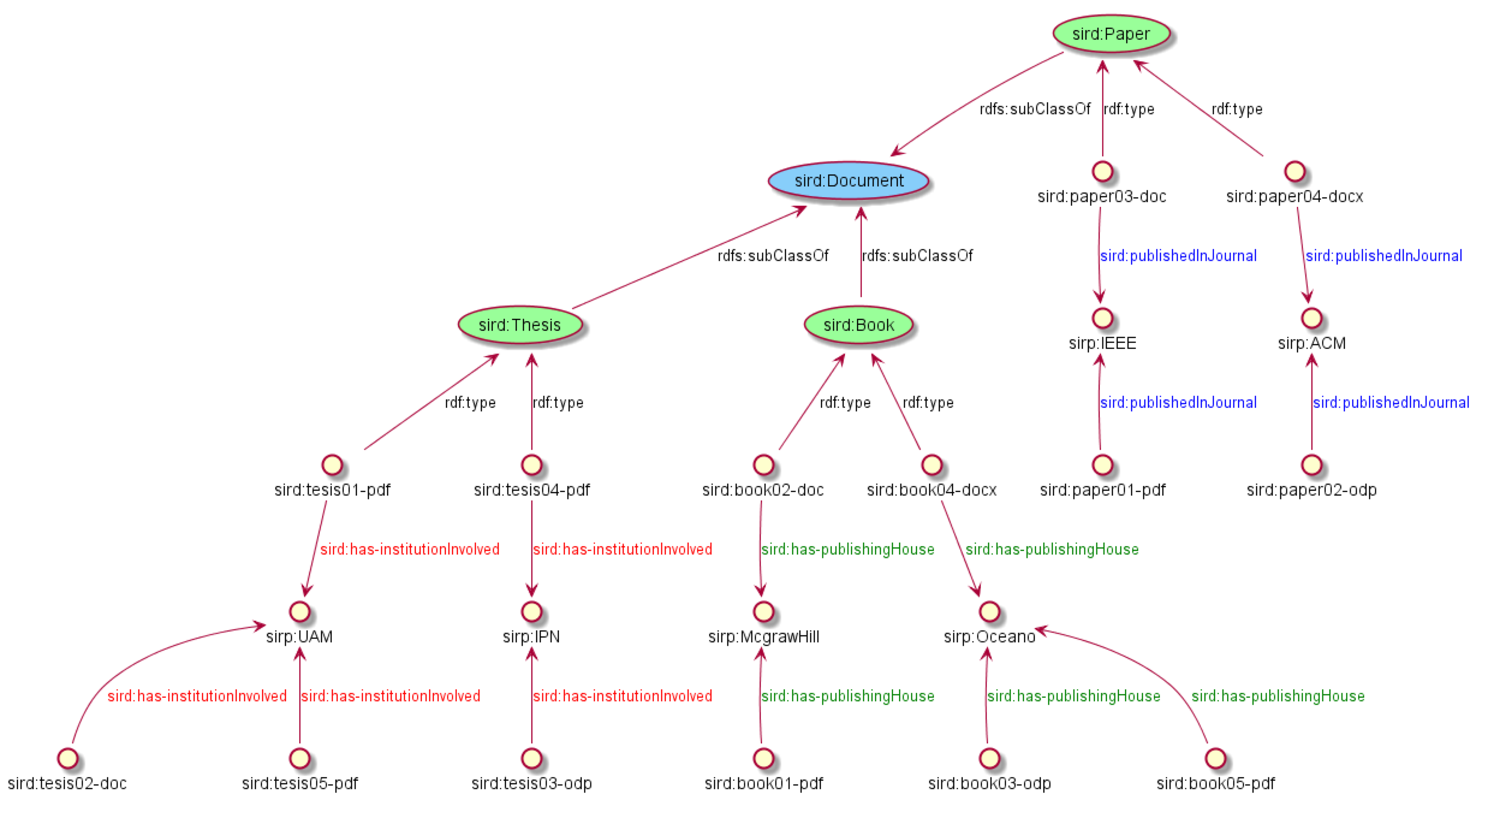
\includegraphics[scale=0.3]{grafoSR}
	\caption{Grafo RDF sin inferencia}
	\end{figure}
	%%%%%%%%%%%%%%%%%%%%%%%%%%%%%%%%%%%
	
	\begin{figure}[htbp]
	\centering
	\subfigure[Consulta sin inferencia]{
	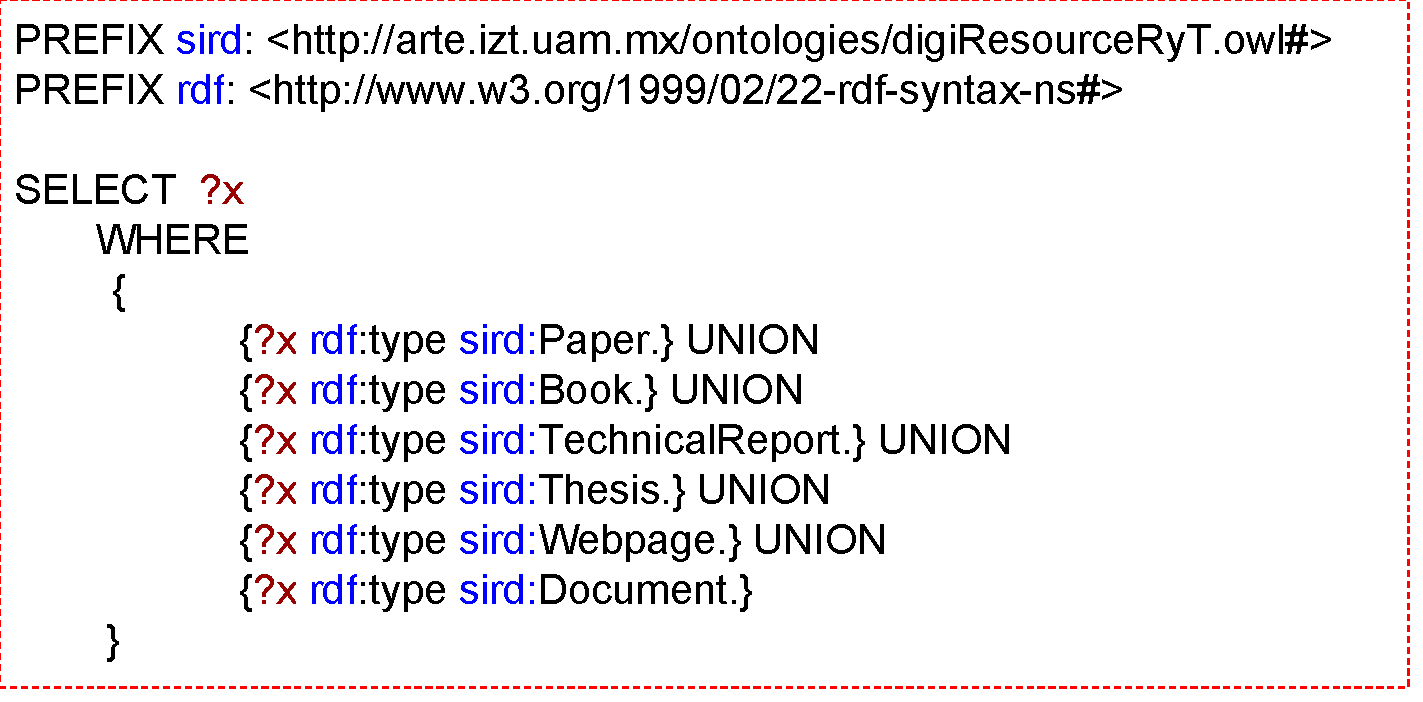
\includegraphics[scale=0.25]{consultaGrafo} 
	}
	\subfigure[Resultados de la consulta]{
	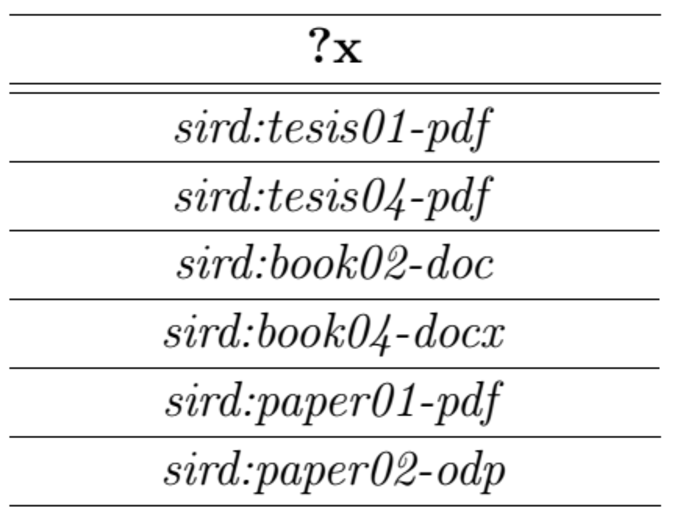
\includegraphics[scale=0.28]{RespQrySI} 
	}
	\end{figure}
	%%%%%%%%%%%%%%%%%%%%%%%%%%%%%%%%%%%
	
	\begin{figure}
	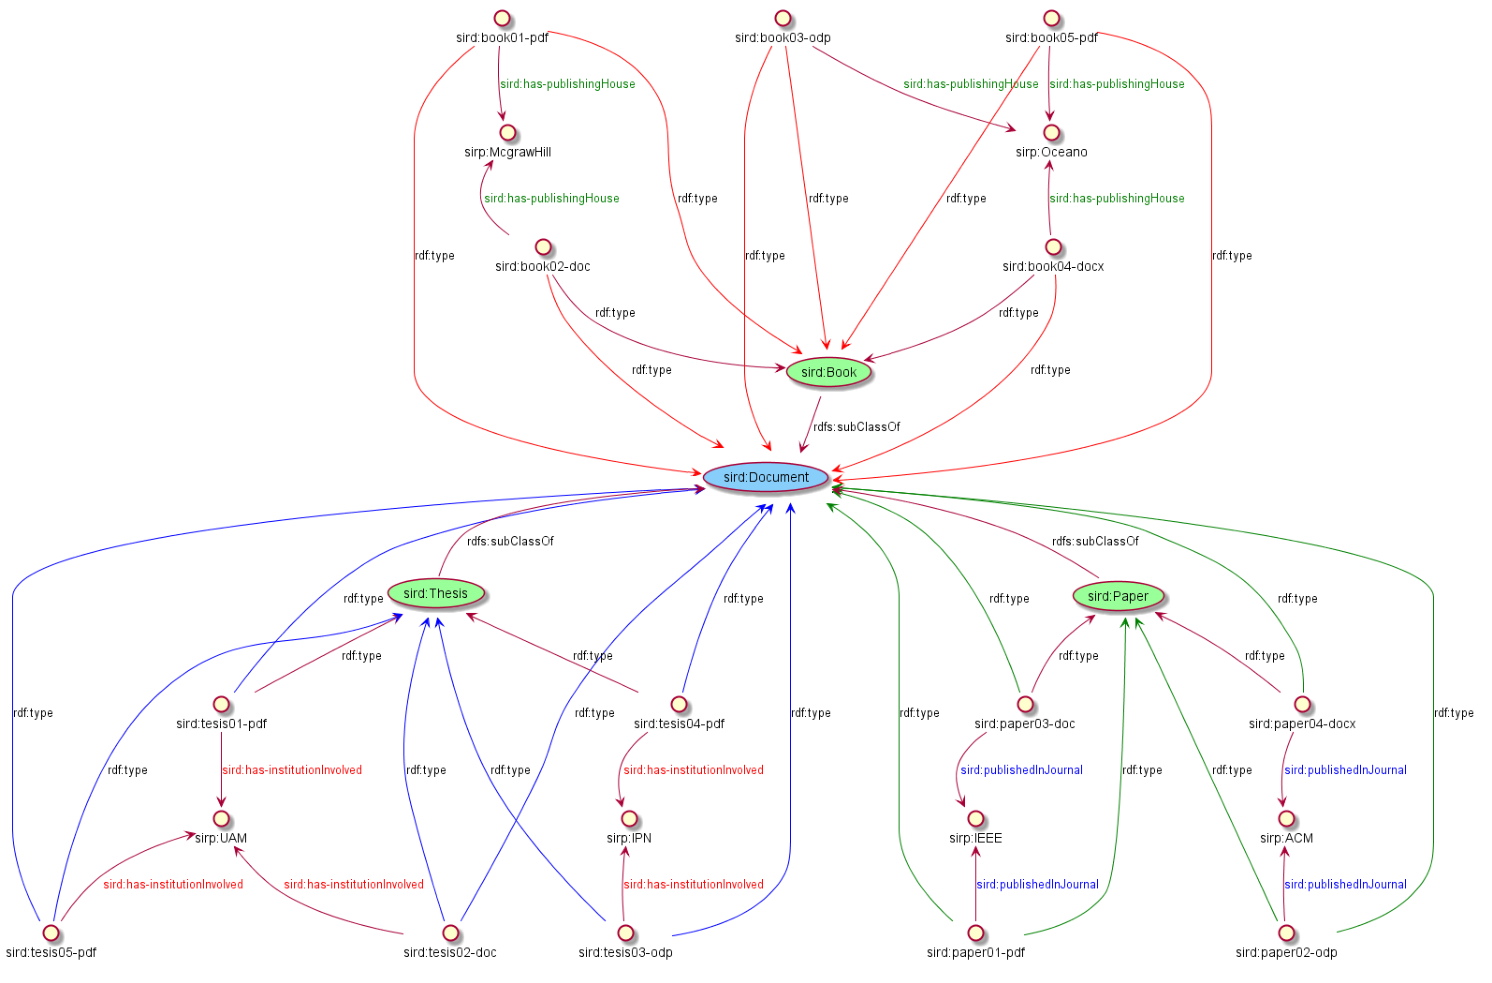
\includegraphics[scale=0.37]{grafoCR}
	\caption{Grafo RDF con inferencia}
	\end{figure}	
	%%%%%%%%%%%%%%%%%%%%%%%%%%%%%%%%%%%
\end{frame}

\subsubsection{Uso de inferencia IV}
\begin{frame}
	\frametitle{Uso de inferencia IV}
	\begin{figure}[htbp]
	\centering
	\subfigure[Consulta con inferencia]{
	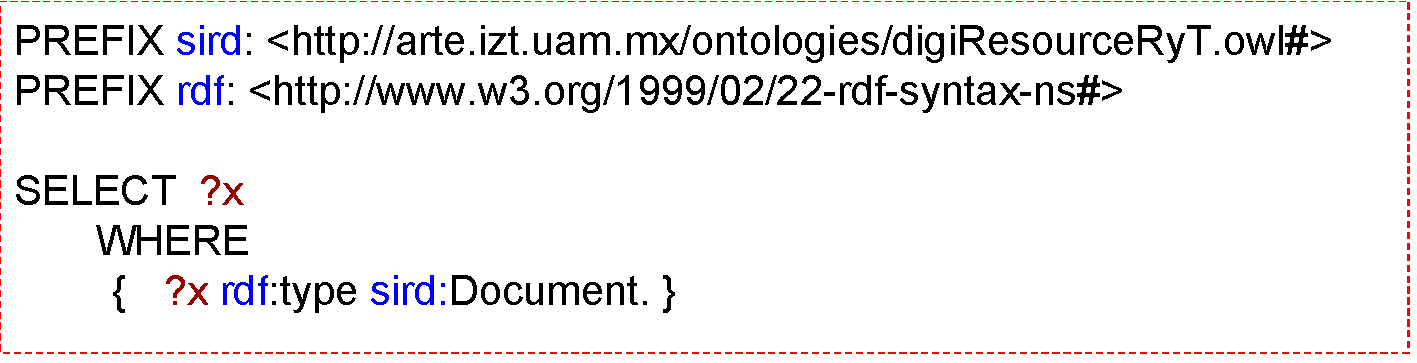
\includegraphics[scale=0.25]{consSimpGrafo} 
	}
	\subfigure[Resultados de la consulta]{
	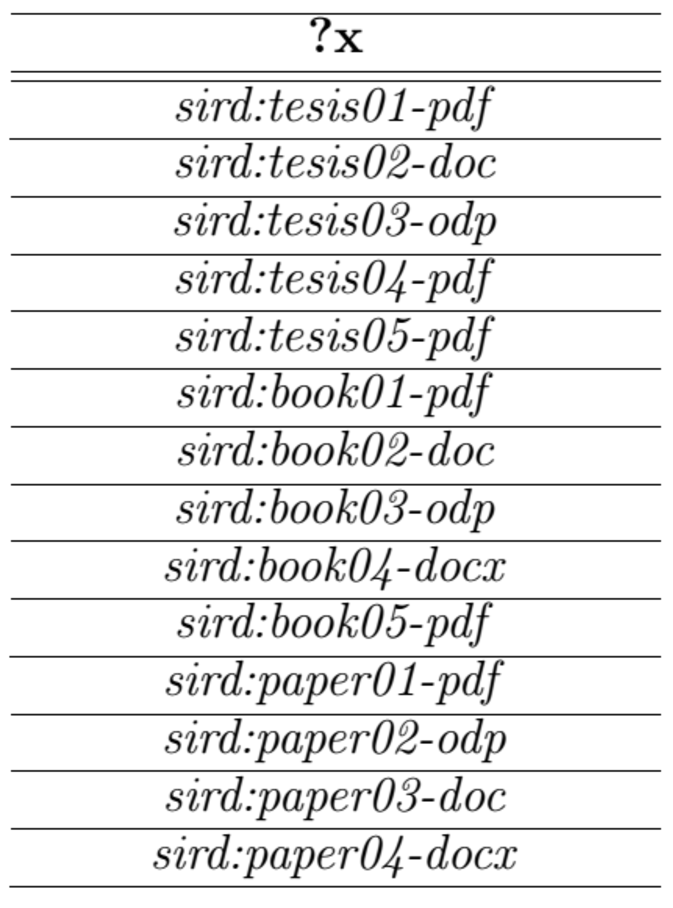
\includegraphics[scale=0.28]{RespQryCI} 
	}
	\end{figure}
\end{frame}


\section{Referencias}
\begin{frame}[allowframebreaks]
\frametitle{Referencias}
\begin{scriptsize} \bibliographystyle{apalike}
\justifying \bibliography{bibliografia}\end{scriptsize}
\end{frame}

\end{document}
